% ============================================================================
%  Dark Halo — Predicting Dark Matter Halo Mass from Baryonic Galaxy Properties
% ============================================================================
\documentclass[12pt, a4paper]{article}

% ── Packages ────────────────────────────────────────────────────────────────
\usepackage[utf8]{inputenc}
\usepackage[T1]{fontenc}
\usepackage{lmodern}
\usepackage{amsmath, amssymb}
\usepackage{booktabs}
\usepackage{graphicx}
\usepackage{hyperref}
\usepackage[margin=2.5cm]{geometry}
\usepackage{caption}
\usepackage{subcaption}
\usepackage{float}
\usepackage{multirow}
\usepackage{siunitx}
\usepackage{xcolor}
\usepackage{natbib}
\usepackage{enumitem}

% ── Graphics path ───────────────────────────────────────────────────────────
\graphicspath{{../artifacts/}}

% ── Custom commands ─────────────────────────────────────────────────────────
\newcommand{\Mhalo}{M_{200\mathrm{c}}}
\newcommand{\logMhalo}{\log_{10}(M_{200\mathrm{c}})}
\newcommand{\Msun}{M_\odot}
\newcommand{\sigmav}{\sigma_v}
\newcommand{\Mstar}{M_\star}
\newcommand{\veldisp}{\sigma_v}

\sisetup{
  group-separator = {,},
  group-minimum-digits = 4,
}

% ── Title ───────────────────────────────────────────────────────────────────
\title{%
  \textbf{Predicting Dark Matter Halo Mass from Baryonic Galaxy Properties}\\[6pt]
  \large An End-to-End Machine Learning Pipeline Using the CAMELS Simulation Suite
}
\author{%
  Syed Abbas Ahmad\\[4pt]
  \normalsize Department of Physics and Applied Sciences\\
  \normalsize Pakistan Institute of Engineering and Applied Sciences (PIEAS)\\[4pt]
  \normalsize \textit{CIS-452: Fundamentals of Machine Learning}
}
\date{\today}

% ============================================================================
\begin{document}
\maketitle

% ~~~~~~~~~~~~~~~~~~~~~~~~~~~~~~~~~~~~~~~~~~~~~~~~~~~~~~~~~~~~~~~~~~~~~~~~~~~~
%  SECTION 1: INTRODUCTION & MOTIVATION
% ~~~~~~~~~~~~~~~~~~~~~~~~~~~~~~~~~~~~~~~~~~~~~~~~~~~~~~~~~~~~~~~~~~~~~~~~~~~~
\section{Introduction}
\label{sec:introduction}

Dark matter halos are the gravitational scaffolds within which visible galaxies form and evolve.  Although they dominate the total mass budget of the universe---constituting roughly 85\% of all matter---their mass cannot be measured through direct electromagnetic observation.  Instead, the mass of a dark matter halo, typically characterised by $\Mhalo$ (the mass enclosed within a sphere whose mean density is 200 times the critical density), must be inferred indirectly, either through gravitational lensing, satellite kinematics, or abundance matching techniques, each of which carries substantial observational uncertainty.

An alternative strategy is to exploit the tight physical correlations that exist between a halo's mass and the baryonic properties of the galaxy it hosts.  The virial theorem implies that a galaxy's velocity dispersion $\sigmav$ scales with the depth of the host halo's gravitational potential well, yielding the approximate relation $M \propto \sigmav^2 R$.  Similarly, the stellar-to-halo mass relation (SHMR), a cornerstone of galaxy formation theory, establishes a monotonic (though non-linear) mapping between a galaxy's stellar mass $\Mstar$ and its host halo mass $\Mhalo$.  These physical relationships suggest that, given a sufficiently rich set of baryonic observables, one may construct a predictive model for halo mass that bypasses the need for direct dark-matter measurements entirely.

Cosmological hydrodynamic simulations provide an ideal laboratory for developing and validating such models.  The CAMELS project (Cosmology and Astrophysics with Machine Learning Simulations) offers a systematic suite of over 4,000 hydrodynamic simulations spanning a wide range of cosmological and astrophysical parameters.  Within CAMELS, the Latin Hypercube (LH) sets---comprising 1,000 simulations per physics model, each run with distinct cosmological parameters $(\Omega_m, \sigma_8)$ and feedback parameters---enable statistically robust model development with built-in variation across the input parameter space.

In this work, we construct an end-to-end machine learning pipeline that predicts $\logMhalo$ from six baryonic features of the central galaxy: stellar mass, gas mass, velocity dispersion, star formation rate, half-mass radius, and an environment proxy based on the distance to the fifth-nearest neighbour.  We benchmark four model classes of increasing complexity---ridge regression, random forest, gradient-boosted trees (XGBoost), and a feed-forward neural network with MC Dropout uncertainty quantification---achieving $R^2 = 0.98$ on held-out test data.  Beyond predictive performance, we employ SHAP feature importance analysis and symbolic regression (PySR) to recover interpretable analytic relations, and we evaluate cross-simulation generalization by testing SIMBA-trained models on IllustrisTNG data.

The remainder of this report is organized as follows.  Section~\ref{sec:data} describes the data acquisition, feature engineering, and leakage-safe splitting strategy.  Section~3 presents an exploratory data analysis characterizing the dataset's statistical properties.  Sections~4 and~5 detail the baseline and neural network models, respectively.  Section~6 provides unified comparative analyses including mass-binned error decomposition and data scaling laws.  Section~7 describes the symbolic regression results, and Section~8 presents the cross-simulation transfer test.  We conclude with a discussion in Section~9.

% ~~~~~~~~~~~~~~~~~~~~~~~~~~~~~~~~~~~~~~~~~~~~~~~~~~~~~~~~~~~~~~~~~~~~~~~~~~~~
%  SECTION 2: DATA & PIPELINE
% ~~~~~~~~~~~~~~~~~~~~~~~~~~~~~~~~~~~~~~~~~~~~~~~~~~~~~~~~~~~~~~~~~~~~~~~~~~~~
\section{Data \& Pipeline}
\label{sec:data}

\subsection{The CAMELS Simulation Suite}
\label{sec:camels}

We use the SIMBA suite within the CAMELS project, accessed via the publicly available FlatHUB API\footnote{\url{https://flathub.flatironinstitute.org/}}.  SIMBA employs the \textsc{Gizmo} meshless finite-mass hydrodynamics code with sub-grid models for star formation, stellar and AGN feedback, and chemical enrichment.  From the Latin Hypercube (LH) design, we download 50 realizations (LH\_0 through LH\_49), each simulated in a $(25\;\mathrm{Mpc}/h)^3$ periodic box with $256^3$ dark matter and $256^3$ gas particles at snapshot~33 (corresponding to redshift $z = 0$).

For each realization, two catalogs are retrieved:

\begin{itemize}[nosep]
  \item \textbf{Group catalog} (halo-level): \num{1012897} total entries across 50 realizations, with a mean of \num{20258} groups per realization (range: \num{17373}--\num{23274}).  Fields include the halo mass $M_{200\mathrm{c}}$, total mass, dark-matter particle count, central subhalo index (\texttt{Group\_FirstSub}), the number of subhalos, and halo position.
  \item \textbf{Subhalo catalog} (galaxy-level): \num{804761} total entries.  Fields include stellar mass, gas mass, velocity dispersion, star formation rate, half-mass radius, and subhalo position.
\end{itemize}

All raw masses are stored in CAMELS internal units of $10^{10}\;\Msun/h$ and are converted to $\Msun/h$ by multiplication by $10^{10}$.  Positions, stored in comoving $\mathrm{kpc}/h$, are converted to $\mathrm{Mpc}/h$ by division by $10^3$.  Velocity dispersions are in $\mathrm{km/s}$ and require no conversion at $z = 0$.

\subsection{Feature Engineering}
\label{sec:features}

The dataset construction pipeline proceeds through five stages, summarized in Table~\ref{tab:pipeline_stages}.

\begin{table}[H]
  \centering
  \caption{Dataset construction stages and row counts.}
  \label{tab:pipeline_stages}
  \begin{tabular}{@{}llr@{}}
    \toprule
    Stage & Description & Rows \\
    \midrule
    Raw download        & All halos and subhalos from 50 LH realizations        & \num{1012897} groups \\
    Quality filter      & Retain only halos with $\geq 100$ dark-matter particles & \num{236097} \\
    Central merge       & Link each halo to its central subhalo via \texttt{Group\_FirstSub} & \num{232563} \\
    Log-target filter   & Remove $M_{200\mathrm{c}} \leq 0$ and compute $\logMhalo$  & \num{228773} \\
    Final dataset       & Clean, finite-valued rows with all features             & \num{228773} \\
    \bottomrule
  \end{tabular}
\end{table}

\paragraph{Central Subhalo Extraction.}
Each halo (friends-of-friends group) may host multiple galaxies (subhalos), of which one is the central galaxy and the remainder are satellites.  Since satellites inhabit a fundamentally different physical environment---they orbit within a larger halo rather than sitting at the potential minimum---including them would introduce a systematic mismatch between baryonic properties and host halo mass.  We therefore restrict the dataset to central subhalos only, identified by the \texttt{Group\_FirstSub} index in the group catalog.  The merge is performed on the composite key (\texttt{simulation\_set\_id}, \texttt{Subhalo\_id} $=$ \texttt{Group\_FirstSub}), yielding \num{232563} matched rows.

\paragraph{Quality Filter.}
Halos resolved with fewer than 100 dark-matter particles are subject to significant numerical noise in their mass estimates and internal properties.  Following standard practice in the simulation literature, we apply a cut $N_{\mathrm{DM}} \geq 100$ (using the \texttt{Group\_LenType\_dm} field), which removes \num{776800} poorly resolved halos (76.7\% of the raw catalog) and retains \num{236097} groups.

\paragraph{Environment Proxy.}
To capture each galaxy's local environment, we compute the distance to its fifth-nearest neighbour (5NN) using a \texttt{scipy.spatial.cKDTree} constructed per realization from the three-dimensional positions of all central subhalos.  This yields the feature \texttt{env\_dist\_5nn} (in $\mathrm{Mpc}/h$), which serves as a density-sensitive proxy: galaxies in denser environments have smaller 5NN distances.

\paragraph{Target Variable.}
The target is defined as $\logMhalo$, where $M_{200\mathrm{c}}$ is in units of $\Msun/h$.  The logarithmic transformation compresses the dynamic range (spanning $10^{7.9}$ to $10^{14.5}\;\Msun/h$) and yields a near-Gaussian target distribution (skewness $= 0.27$, kurtosis $= 1.08$), facilitating regression.

The final dataset comprises \num{228773} rows and nine baryonic features plus the target.  Feature descriptions and units are given in Table~\ref{tab:features}.

\begin{table}[H]
  \centering
  \caption{Feature set used for modeling.  The six modeling features (above the rule) are used in all models; the three spatial position features (below the rule) are excluded from models after EDA confirmed their negligible correlation with halo mass ($|r| < 0.02$).}
  \label{tab:features}
  \begin{tabular}{@{}llll@{}}
    \toprule
    Feature & Symbol & Unit & Description \\
    \midrule
    \texttt{stellar\_mass}   & $\Mstar$     & $\Msun/h$       & Stellar mass of the central subhalo \\
    \texttt{gas\_mass}       & $M_\mathrm{gas}$      & $\Msun/h$       & Gas mass of the central subhalo \\
    \texttt{vel\_disp}       & $\sigmav$    & $\mathrm{km/s}$ & 1D velocity dispersion \\
    \texttt{sfr}             & SFR          & $\Msun/\mathrm{yr}$ & Instantaneous star formation rate \\
    \texttt{half\_mass\_rad} & $r_{1/2}$    & $\mathrm{kpc}/h$     & Stellar half-mass radius \\
    \texttt{env\_dist\_5nn}  & $d_{5\mathrm{NN}}$  & $\mathrm{Mpc}/h$     & Distance to 5th-nearest central subhalo \\
    \midrule
    \texttt{pos\_x, pos\_y, pos\_z} & $(x,y,z)$ & $\mathrm{Mpc}/h$ & Comoving spatial position (excluded from models) \\
    \bottomrule
  \end{tabular}
\end{table}

\subsection{Leakage-Safe Data Splitting}
\label{sec:splitting}

A critical design consideration in any machine learning study using cosmological simulations is the prevention of \emph{data leakage} across the train--validation--test boundary.  Within a single CAMELS realization, all halos share the same cosmological parameters $(\Omega_m, \sigma_8)$ and feedback parameters $(A_\mathrm{SN1}, A_\mathrm{SN2}, A_\mathrm{AGN1}, A_\mathrm{AGN2})$.  A naive random split at the row level would allow the model to memorize realization-specific correlations---for example, a particular $(\Omega_m, \sigma_8)$ combination that systematically shifts all halo masses---and thus report inflated test-set performance that would not transfer to genuinely unseen cosmologies.

To prevent this, we split at the \emph{realization level}.  The 50 realization IDs are shuffled with a fixed random seed ($s = 42$) and partitioned into three non-overlapping groups:

\begin{table}[H]
  \centering
  \caption{Data split by CAMELS realization, ensuring zero overlap in cosmological parameters across splits.}
  \label{tab:splits}
  \begin{tabular}{@{}lrrrrr@{}}
    \toprule
    Split & Realizations & Rows & $\overline{\logMhalo}$ & $\sigma_{\logMhalo}$ & Range \\
    \midrule
    Train & 35 & \num{159143} & 9.987 & 0.733 & $[7.86, 14.52]$ \\
    Val   &  8 &  \num{36863} & 10.043 & 0.676 & $[8.11, 14.12]$ \\
    Test  &  7 &  \num{32767} & 9.994 & 0.734 & $[7.89, 13.74]$ \\
    \midrule
    Total & 50 & \num{228773} & --- & --- & --- \\
    \bottomrule
  \end{tabular}
\end{table}

The target distribution is well-balanced across splits: the mean $\logMhalo$ varies by less than 0.06~dex between any two splits, and the standard deviations agree to within 0.06~dex (Table~\ref{tab:splits}).  The validation set is used for hyperparameter tuning and early stopping; the test set is reserved for final evaluation and is never used during model development.

We verify the integrity of this split by confirming that no realization ID appears in more than one split.  The specific realization assignments are recorded in a machine-readable manifest (\texttt{split\_manifest.json}) for full reproducibility.

% ~~~~~~~~~~~~~~~~~~~~~~~~~~~~~~~~~~~~~~~~~~~~~~~~~~~~~~~~~~~~~~~~~~~~~~~~~~~~
%  SECTION 3: EXPLORATORY DATA ANALYSIS
% ~~~~~~~~~~~~~~~~~~~~~~~~~~~~~~~~~~~~~~~~~~~~~~~~~~~~~~~~~~~~~~~~~~~~~~~~~~~~
\section{Exploratory Data Analysis}
\label{sec:eda}

Before fitting any model, we conduct a systematic exploratory analysis to characterize the statistical properties of the dataset, identify potential pathologies, and inform preprocessing decisions.  The EDA comprises four stages: a missingness audit, distributional profiling, correlation analysis, and out-of-distribution (OOD) detection.

\subsection{Data Quality Audit}
\label{sec:missingness}

A column-by-column scan confirms that the dataset contains exactly zero NaN and zero Inf values across all ten features and the target variable ($n = \num{228773}$ rows $\times$ 10 columns).  This is expected for simulation-derived catalogs, which, unlike observational data, are not subject to missing detections or measurement dropouts.  No imputation or data-cleaning procedures are therefore required.

\subsection{Feature Distributions}
\label{sec:distributions}

Table~\ref{tab:dist_stats} summarizes the first four moments of each feature.  Several patterns warrant attention:

\begin{table}[H]
  \centering
  \caption{Distributional statistics of all features and the target.  Skewness and excess kurtosis are reported for the raw (untransformed) values.}
  \label{tab:dist_stats}
  \begin{tabular}{@{}lrrrrr@{}}
    \toprule
    Feature & Mean & Std & Median & Skew & Kurtosis \\
    \midrule
    $\logMhalo$ [\text{dex}]       & 9.997 & 0.724 & 9.987 & 0.27 & 1.08 \\
    $\Mstar$ [$\Msun/h$]           & $1.28 \times 10^{9}$ & $2.08 \times 10^{10}$ & $0$ & 83.42 & \num{12430} \\
    $M_\mathrm{gas}$ [$\Msun/h$]   & $5.02 \times 10^{9}$ & $1.01 \times 10^{11}$ & $2.53 \times 10^{8}$ & 124.50 & \num{25043} \\
    $\sigmav$ [\text{km/s}]         & 27.45 & 24.79 & 18.25 & 3.52 & 26.93 \\
    SFR [$\Msun/\mathrm{yr}$]       & 0.069 & 0.956 & 0.0 & 143.92 & \num{32739} \\
    $r_{1/2}$ [\text{kpc/}$h$]      & 25.63 & 15.63 & 23.34 & 6.54 & 86.05 \\
    $d_{5\mathrm{NN}}$ [\text{Mpc/}$h$] & 1.150 & 0.527 & 1.038 & 1.47 & 3.63 \\
    \midrule
    $x, y, z$ [\text{Mpc/}$h$]     & $\sim$12.4 & $\sim$7.3 & $\sim$12.3 & $\sim$0.03 & $-$1.23 \\
    \bottomrule
  \end{tabular}
\end{table}

\paragraph{Extreme skewness in mass and SFR features.}
Stellar mass, gas mass, and star formation rate exhibit skewness values of 83.4, 124.5, and 143.9, respectively, with excess kurtosis exceeding $10^4$.  This reflects the fact that most halos in the dataset host low-mass galaxies with little or no star formation, while a small number of massive systems dominate the upper tail.  To mitigate the impact of these heavy tails on gradient-based learners, we apply a $\log_{10}(x + 1)$ transformation to stellar mass and gas mass before fitting linear and tree models.

\paragraph{Near-Gaussian target.}
The target variable $\logMhalo$ has modest skewness (0.27) and kurtosis (1.08), confirming that the logarithmic transformation yields a well-behaved, nearly symmetric distribution suitable for squared-error regression objectives without further transformation.

\paragraph{Uniform spatial positions.}
The three position coordinates are uniformly distributed across the simulation box ($\text{skew} \approx 0.03$, $\text{kurtosis} \approx -1.23$), as expected from the periodic boundary conditions.

Figure~\ref{fig:distributions} displays histograms for all nine features, with log-transformed axes for the skewed mass variables.  The target distribution, stratified by train/val/test split, is shown in Figure~\ref{fig:target_dist}.

\begin{figure}[H]
  \centering
  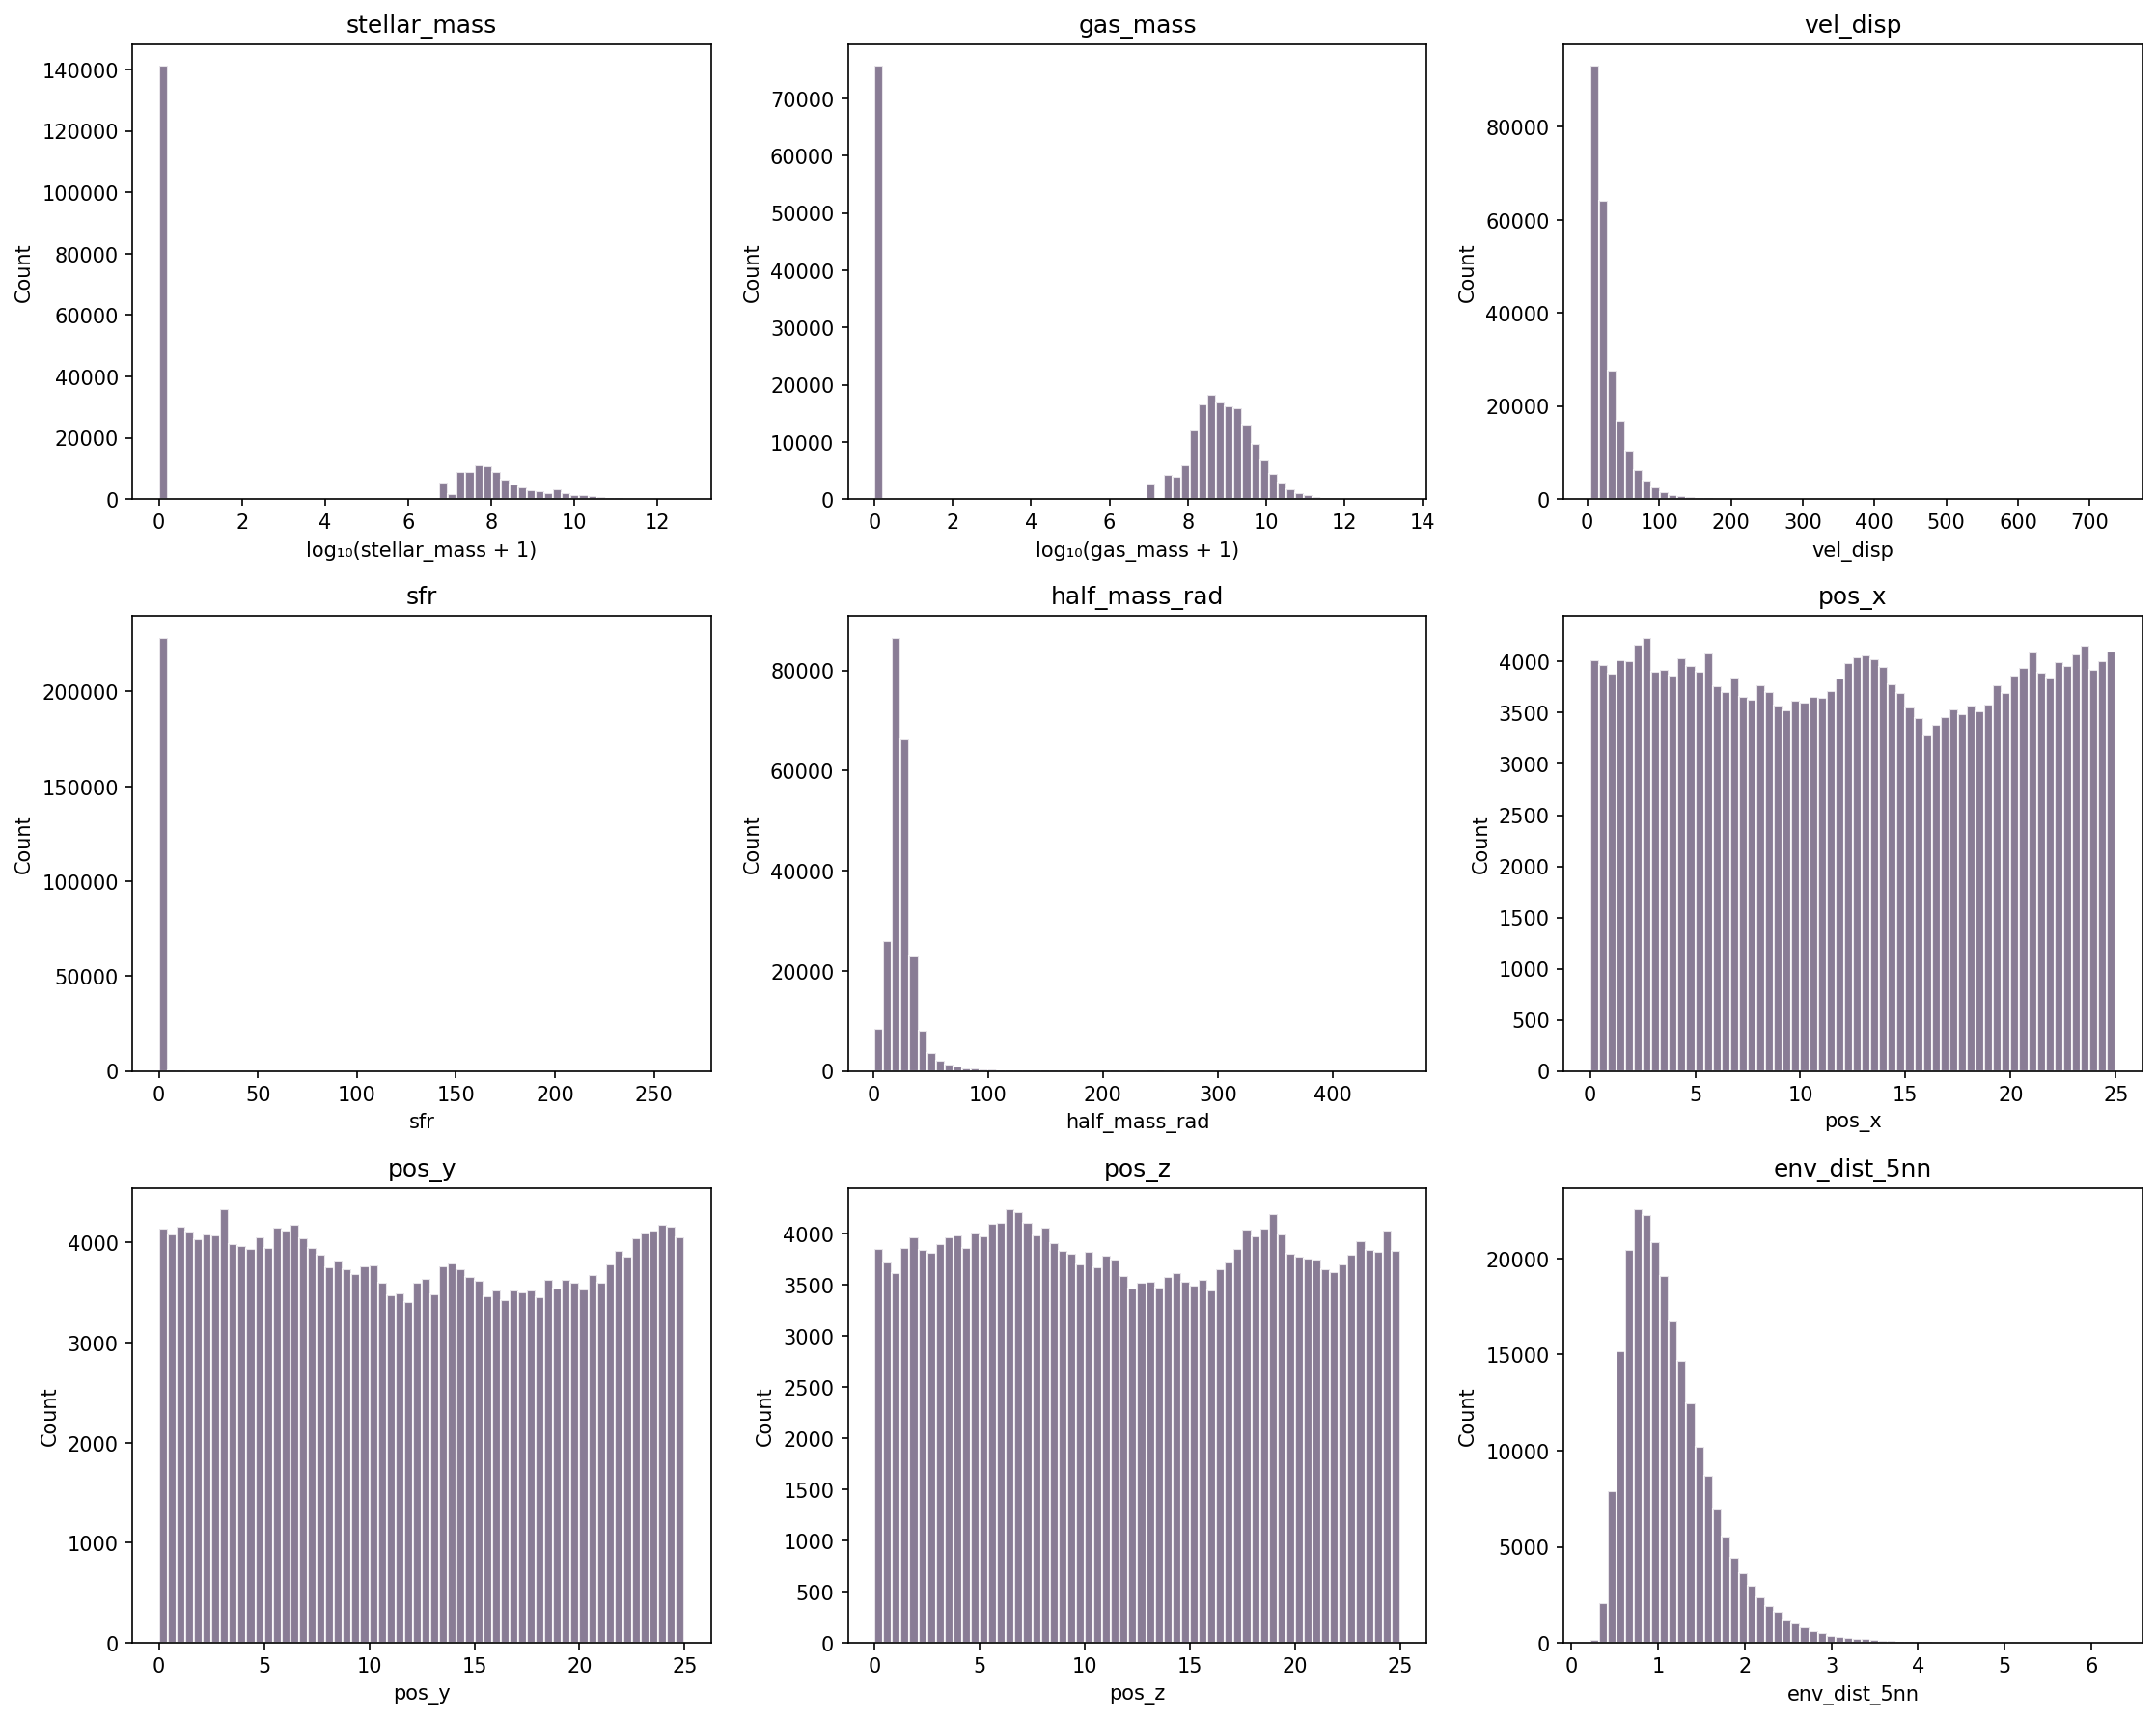
\includegraphics[width=0.95\textwidth]{step4_eda/feature_distributions.png}
  \caption{Feature distributions across all \num{228773} rows.  Mass features (top row) are plotted on log-scaled axes to reveal the full dynamic range.  Velocity dispersion (middle-left) displays a right-skewed unimodal shape.}
  \label{fig:distributions}
\end{figure}

\begin{figure}[H]
  \centering
  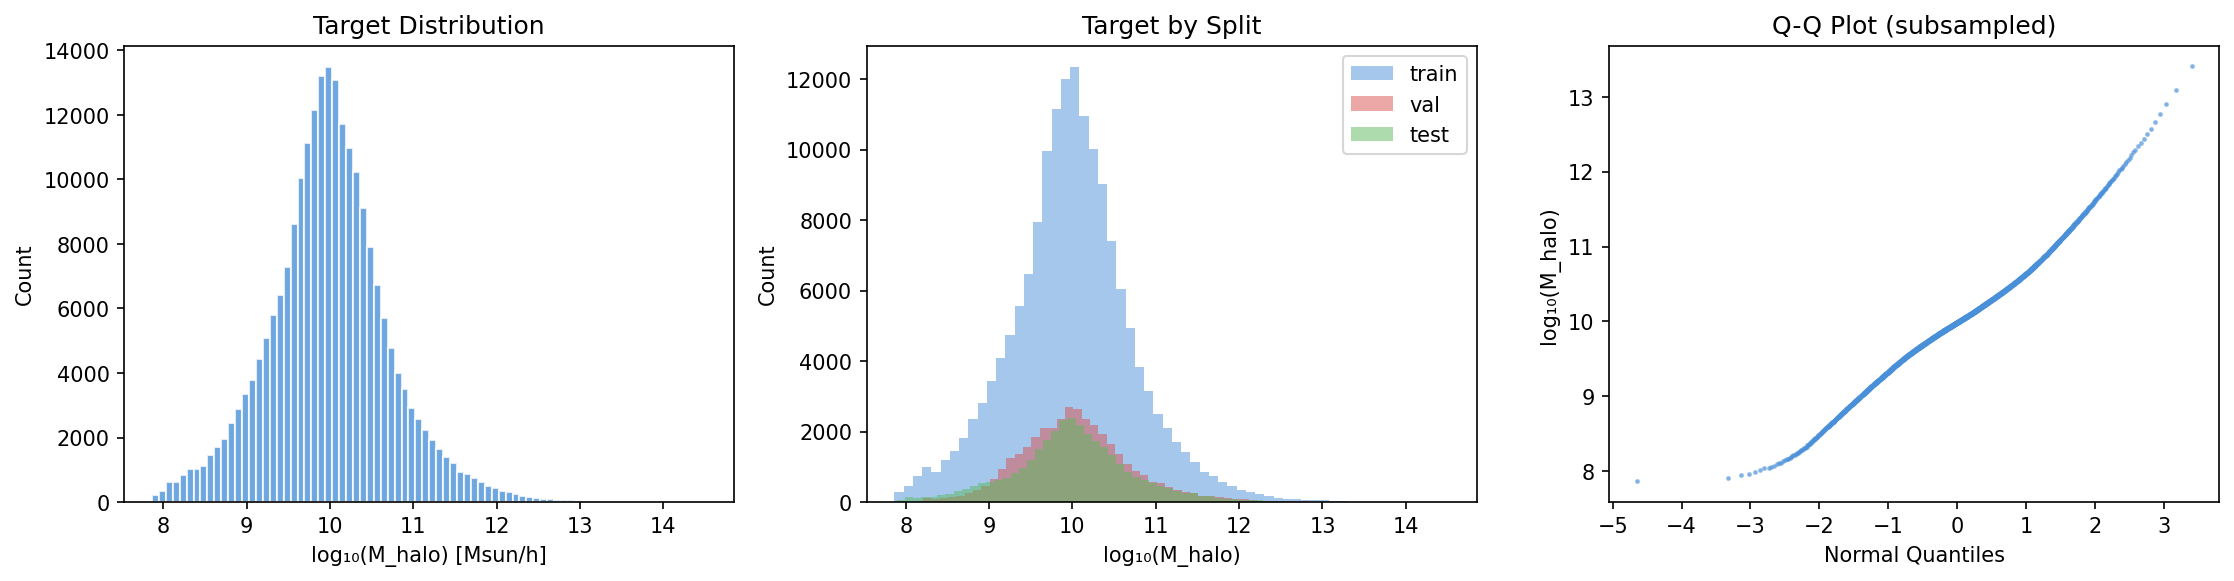
\includegraphics[width=0.75\textwidth]{step4_eda/target_distribution.png}
  \caption{Target distribution ($\logMhalo$) stratified by data split.  The three splits exhibit closely matched means ($\Delta\bar{y} < 0.06$~dex) and standard deviations ($\Delta\sigma < 0.06$~dex), confirming that the realization-level splitting strategy preserves target balance.}
  \label{fig:target_dist}
\end{figure}

\subsection{Correlation Analysis}
\label{sec:correlations}

Table~\ref{tab:correlations} reports the Pearson correlation coefficient $r$ between each feature and the target $\logMhalo$.

\begin{table}[H]
  \centering
  \caption{Pearson correlation of each feature with $\logMhalo$.  Features are sorted by $|r|$.}
  \label{tab:correlations}
  \begin{tabular}{@{}lrl@{}}
    \toprule
    Feature & $r$ & Interpretation \\
    \midrule
    $\sigmav$              & $+0.852$ & Dominant predictor (virial theorem) \\
    $r_{1/2}$              & $+0.313$ & Moderate positive (size--mass relation) \\
    $\Mstar$               & $+0.211$ & Positive (SHMR) \\
    SFR                    & $+0.176$ & Weak positive \\
    $M_\mathrm{gas}$       & $+0.149$ & Weak positive \\
    $d_{5\mathrm{NN}}$     & $-0.114$ & Weak negative (assembly bias) \\
    $x, y, z$              & $< 0.013$ & Negligible (position-independent) \\
    \bottomrule
  \end{tabular}
\end{table}

Velocity dispersion exhibits the strongest linear correlation ($r = +0.852$), consistent with its role as a virial mass proxy: for a virialized system, $\Mhalo \propto \sigmav^2 R$, where $R$ is the halo virial radius.  The residual scatter around the $\sigmav$--$M$ relation motivates the inclusion of additional features and the use of non-linear models.

Stellar mass shows a positive but modest correlation ($r = +0.211$) in its raw form.  This underestimate of its true predictive power stems from the extreme skewness; after log-transformation, the Pearson correlation with the log-target rises substantially, reflecting the well-known stellar-to-halo mass relation (SHMR).

The three spatial position coordinates have correlations $|r| < 0.013$, confirming that halo mass is independent of position within the simulation box.  These features are therefore excluded from all subsequent models.

The environment proxy $d_{5\mathrm{NN}}$ shows a weak negative correlation ($r = -0.114$): galaxies in denser environments (smaller $d_{5\mathrm{NN}}$) tend to inhabit more massive halos.  This is consistent with the expected assembly bias signal, whereby massive halos cluster more strongly.

Figure~\ref{fig:corr_matrix} shows the full feature--feature and feature--target correlation matrix, and Figure~\ref{fig:scatter} presents bivariate scatter plots of each feature against the target.

\begin{figure}[H]
  \centering
  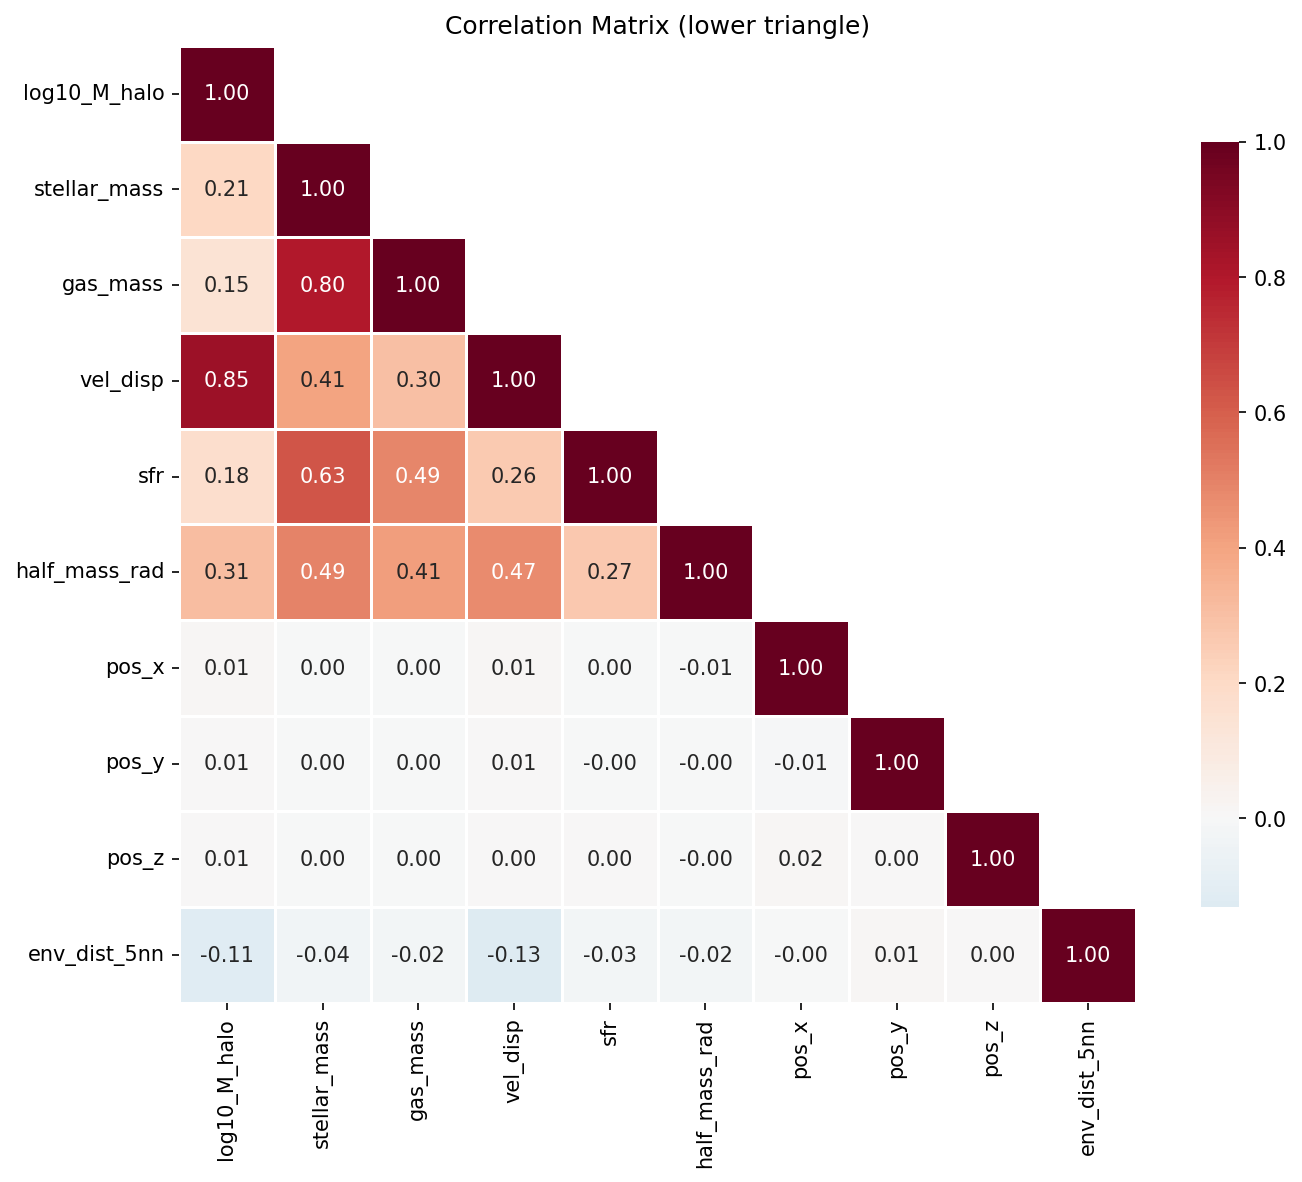
\includegraphics[width=0.85\textwidth]{step4_eda/correlation_matrix.png}
  \caption{Pearson correlation heatmap (left) and feature--target bar chart (right).  $\sigmav$ dominates with $r = +0.852$.  Spatial coordinates are near zero.}
  \label{fig:corr_matrix}
\end{figure}

\begin{figure}[H]
  \centering
  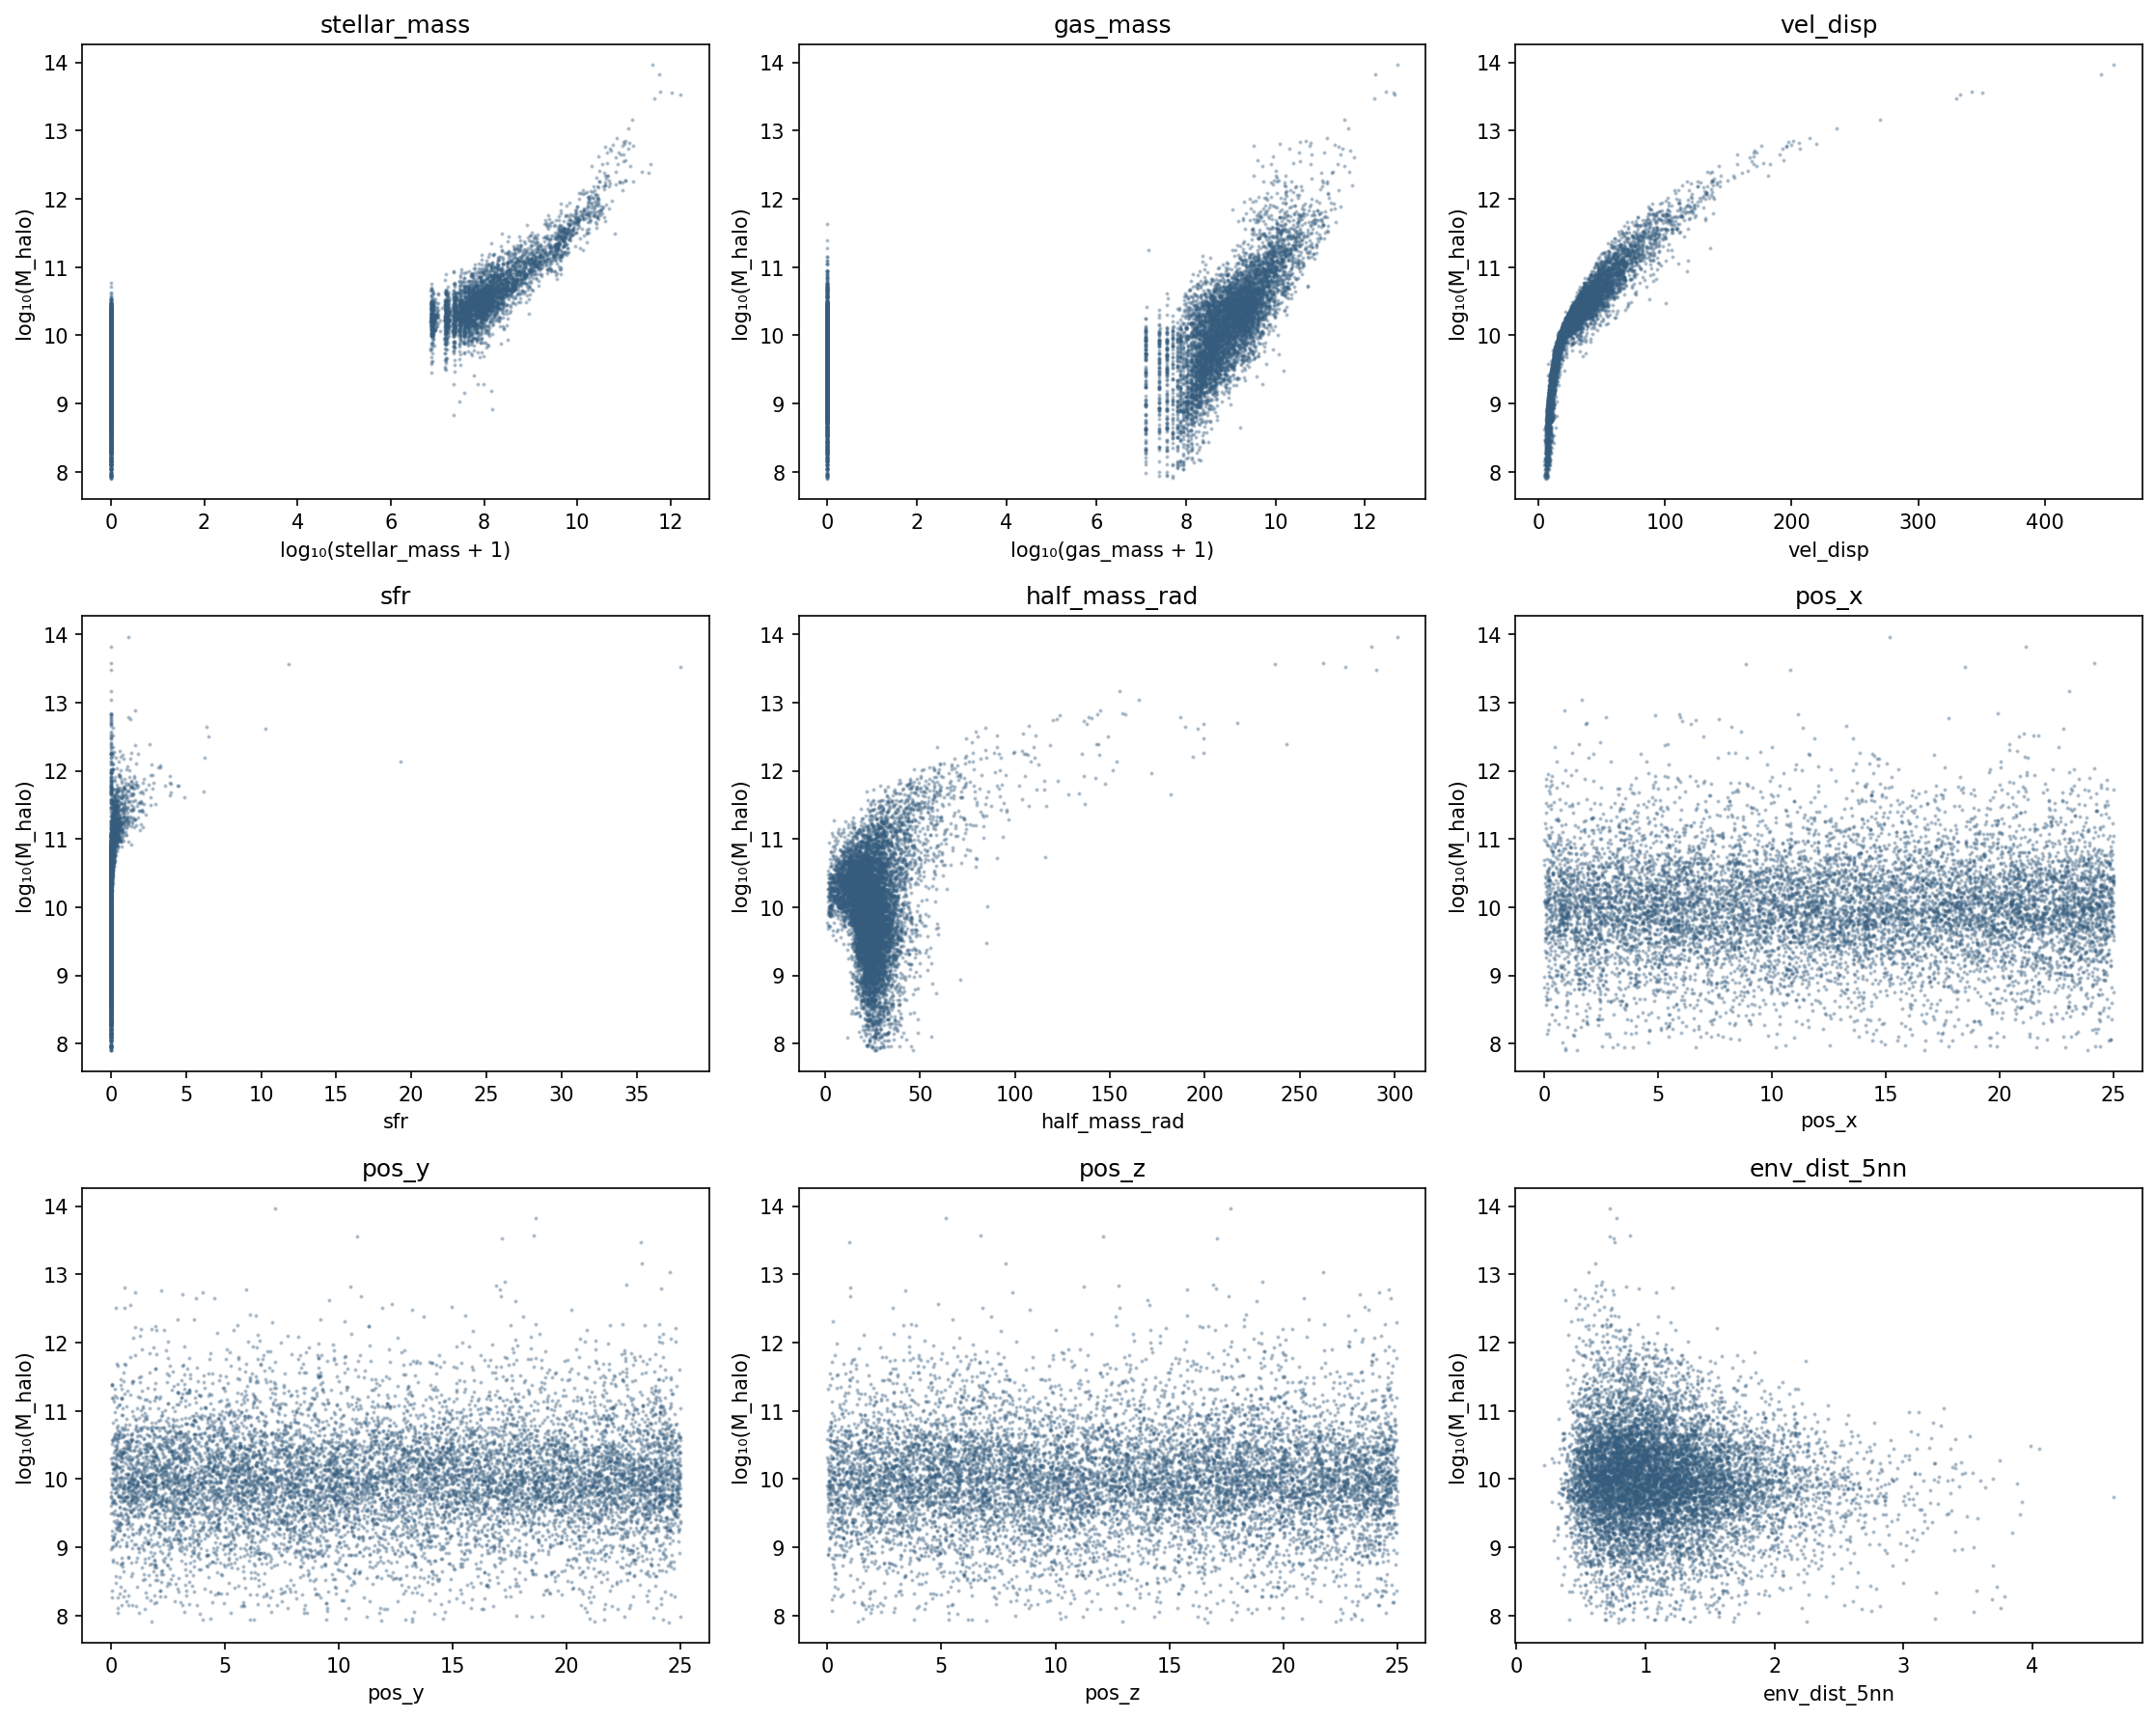
\includegraphics[width=0.95\textwidth]{step4_eda/feature_vs_target.png}
  \caption{Scatter plots of each feature versus $\logMhalo$ (10,000-row subsample for readability).  The $\sigmav$--$M$ panel reveals a tight, monotonic, non-linear relationship.  Mass features are shown on log-transformed axes.}
  \label{fig:scatter}
\end{figure}

\subsection{Out-of-Distribution Detection}
\label{sec:ood}

To assess whether the dataset contains anomalous galaxies that might disproportionately influence model training, we apply an Isolation Forest (scikit-learn, contamination = 5\%) trained on the six modeling features of the training set.  The detector flags \num{4654} out of \num{228773} rows (2.03\%) as potential outliers.

Critically, the OOD rate is consistent across splits: 2.00\% in training ($n = \num{3183}$), 2.15\% in validation ($n = 792$), and 2.07\% in test ($n = 679$).  This uniformity confirms that the realization-level split does not introduce systematic distributional shift, and that no split is disproportionately contaminated by anomalous objects.

We choose to \emph{retain} the flagged outliers in the training set for two reasons: (i)~the OOD rate is sufficiently low that removal would negligibly affect model training, and (ii)~in a physical context, these ``outliers'' may represent genuinely extreme objects (e.g., cluster-scale halos or quenched low-mass systems) that the model should learn to handle.

\begin{figure}[H]
  \centering
  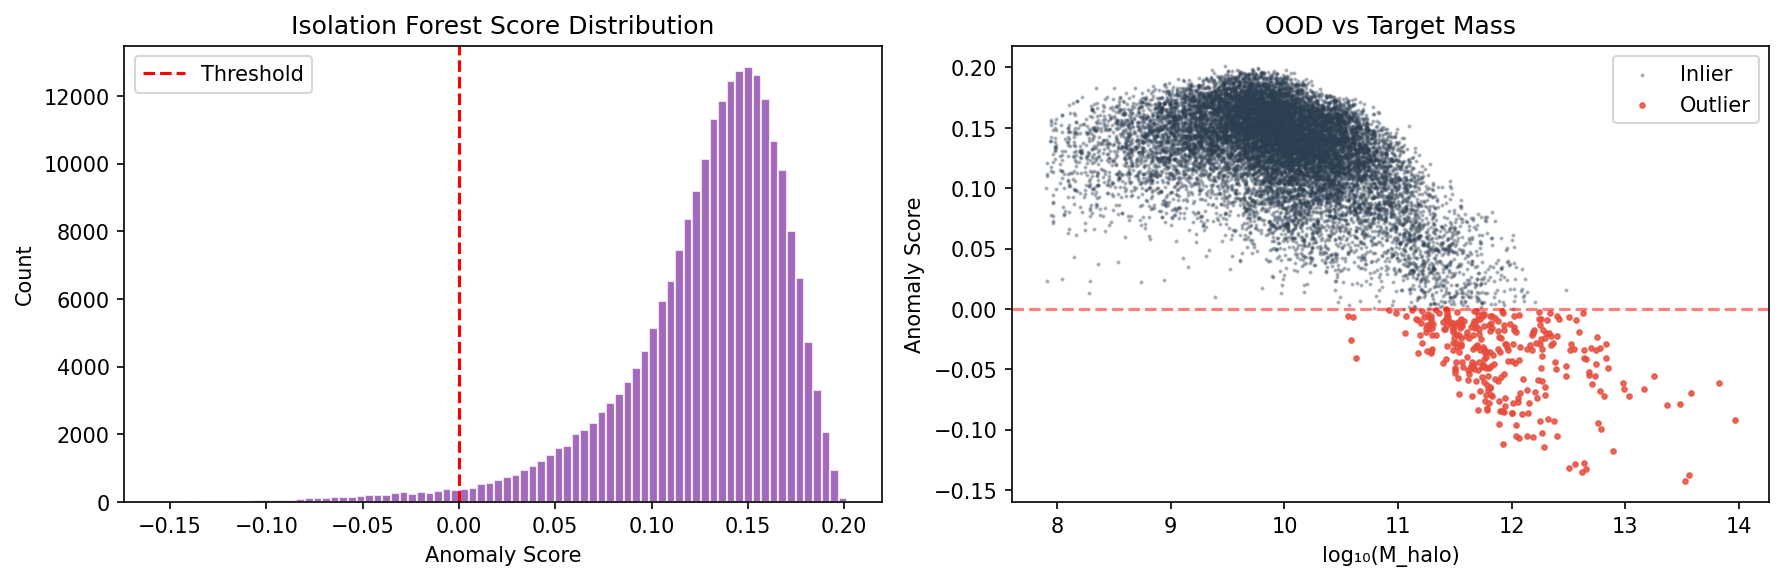
\includegraphics[width=0.75\textwidth]{step4_eda/isolation_forest_ood.png}
  \caption{Isolation Forest OOD detection.  2.03\% of the dataset (4,654 rows) is flagged, with consistent rates across train (2.00\%), validation (2.15\%), and test (2.07\%) splits.}
  \label{fig:ood}
\end{figure}


% ~~~~~~~~~~~~~~~~~~~~~~~~~~~~~~~~~~~~~~~~~~~~~~~~~~~~~~~~~~~~~~~~~~~~~~~~~~~~
%  SECTION 4: BASELINE MODELS
% ~~~~~~~~~~~~~~~~~~~~~~~~~~~~~~~~~~~~~~~~~~~~~~~~~~~~~~~~~~~~~~~~~~~~~~~~~~~~
\section{Baseline Models}
\label{sec:baselines}

We establish model performance across two tiers of complexity: a linear regression baseline (Section~\ref{sec:linear}) and tree-ensemble models (Section~\ref{sec:trees}).  All models are trained on the same six engineered features ($\log_{10}(\Mstar + 1)$, $\log_{10}(M_\mathrm{gas} + 1)$, $\sigmav$, SFR, $r_{1/2}$, $d_{5\mathrm{NN}}$), with spatial position coordinates excluded per the EDA findings of Section~\ref{sec:correlations}.

\subsection{Linear and Ridge Regression}
\label{sec:linear}

As a lower-bound baseline, we fit ordinary least squares (OLS) and ridge regression with two regularization strengths ($\alpha \in \{1.0, 10.0\}$).  All features are standardized via \texttt{StandardScaler} (zero mean, unit variance) fitted on the training set and applied to validation and test sets without refitting, ensuring no information leakage.  Mass features are log-transformed ($\log_{10}(x + 1)$) prior to scaling.

\begin{table}[H]
  \centering
  \caption{Linear and ridge regression performance across splits.  OLS and Ridge($\alpha = 1$) produce numerically identical results, indicating that the data is well-conditioned with negligible collinearity.}
  \label{tab:linear_results}
  \begin{tabular}{@{}llccc@{}}
    \toprule
    Model & Split & RMSE & MAE & $R^2$ \\
    \midrule
    \multirow{3}{*}{OLS / Ridge($\alpha=1$)}
      & Train & 0.3554 & 0.2628 & 0.7648 \\
      & Val   & 0.3034 & 0.2309 & 0.7988 \\
      & Test  & 0.3640 & 0.2748 & 0.7537 \\
    \midrule
    \multirow{3}{*}{Ridge($\alpha=10$)}
      & Train & 0.3554 & 0.2628 & 0.7648 \\
      & Val   & 0.3034 & 0.2309 & 0.7988 \\
      & Test  & 0.3640 & 0.2748 & 0.7537 \\
    \bottomrule
  \end{tabular}
\end{table}

The linear model achieves a test $R^2$ of 0.7537 with an RMSE of 0.3640~dex.  Notably, increasing the regularization strength from $\alpha = 1$ to $\alpha = 10$ produces no detectable change in performance (Table~\ref{tab:linear_results}), confirming that the six features do not suffer from multicollinearity and that the least-squares problem is well-posed.

Table~\ref{tab:linear_coefficients} presents the standardized regression coefficients, which reveal a clear physical hierarchy:

\begin{table}[H]
  \centering
  \caption{Standardized coefficients from Ridge($\alpha = 1$), sorted by absolute magnitude.  After standardization, coefficients are directly comparable in terms of per-standard-deviation effect on the predicted target.}
  \label{tab:linear_coefficients}
  \begin{tabular}{@{}lr@{}}
    \toprule
    Feature & Coefficient \\
    \midrule
    $\sigmav$              & $+0.494$ \\
    $\log_{10}(\Mstar + 1)$ & $+0.170$ \\
    $\log_{10}(M_\mathrm{gas} + 1)$ & $+0.064$ \\
    $r_{1/2}$              & $-0.043$ \\
    SFR                    & $-0.018$ \\
    $d_{5\mathrm{NN}}$     & $-0.005$ \\
    \bottomrule
  \end{tabular}
\end{table}

Velocity dispersion dominates the linear prediction ($\beta = +0.494$), contributing roughly three times more than stellar mass ($\beta = +0.170$) per unit standard deviation.  Gas mass provides a modest additional signal ($\beta = +0.064$), while the remaining three features contribute marginally.  The negative coefficient for $r_{1/2}$ ($-0.043$) may reflect the fact that, at fixed velocity dispersion, more compact galaxies tend to reside in slightly more massive halos.

Diagnostic plots (Figures~\ref{fig:linear_pred} and~\ref{fig:linear_resid}) reveal qualitative limitations of the linear model: the predicted-vs-true scatter shows systematic curvature at both the low-mass and high-mass tails, and the residual distribution exhibits heavier tails than a Gaussian, indicating that the $\sigmav$--$\Mhalo$ relationship contains non-linear structure that a linear model cannot capture.

\begin{figure}[H]
  \centering
  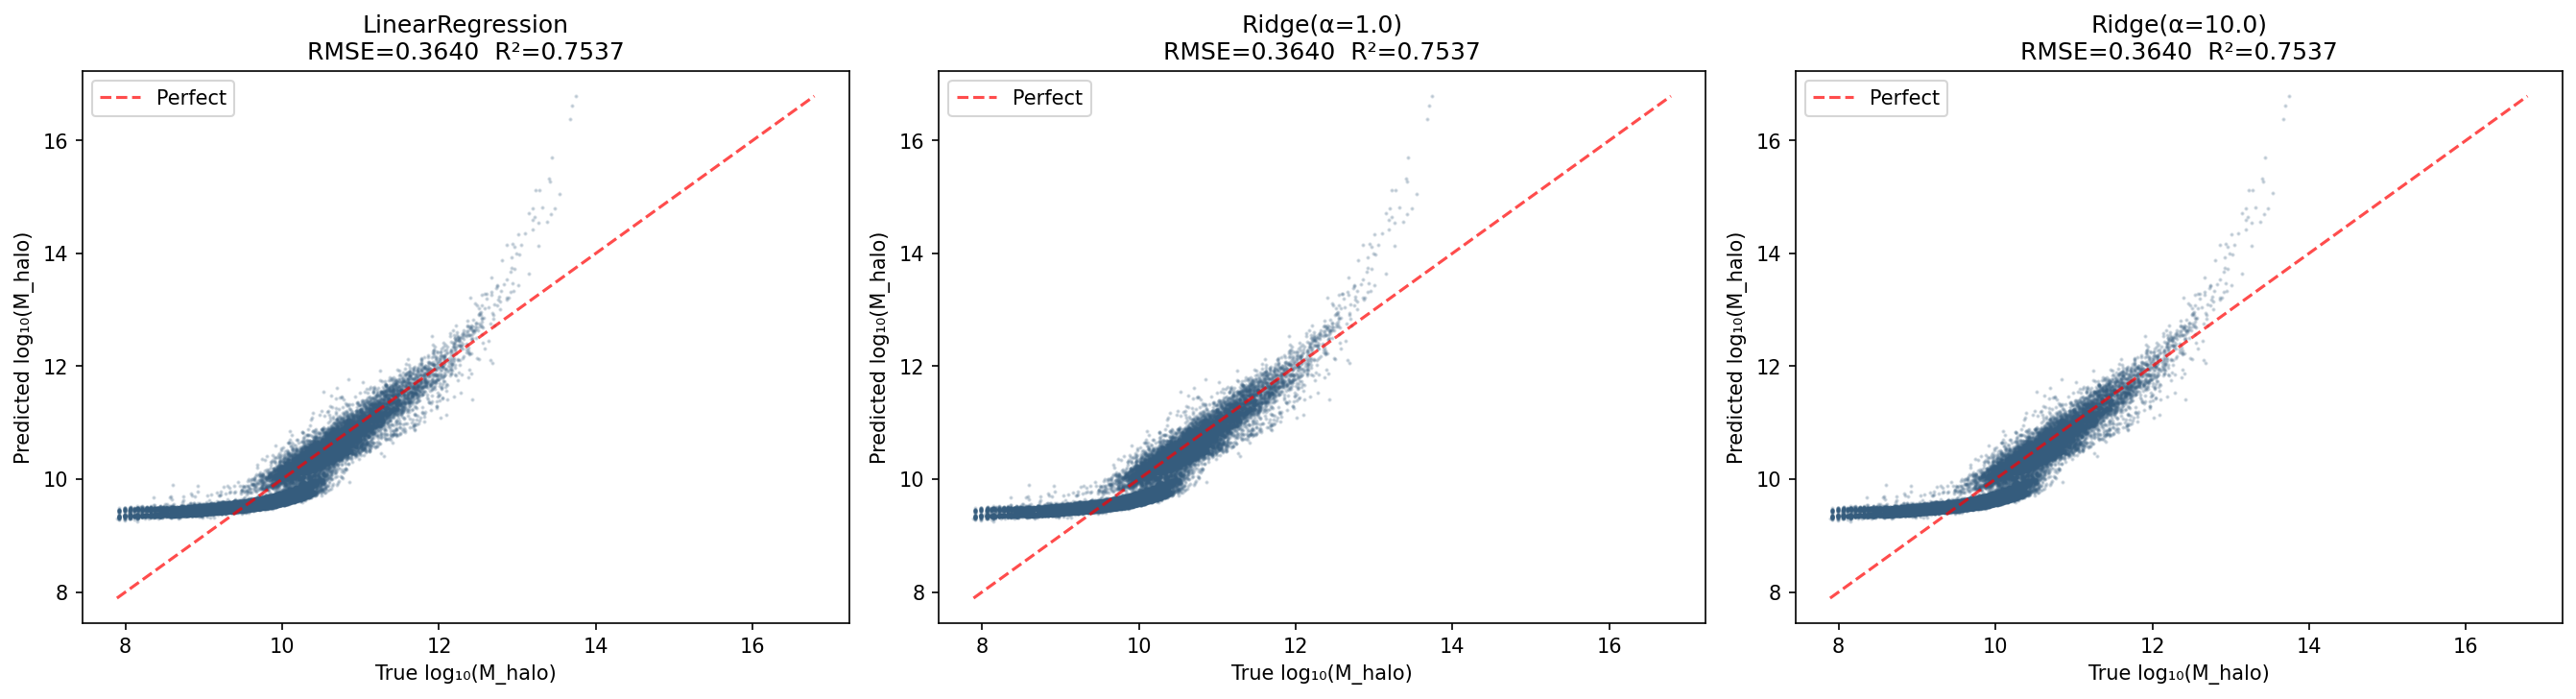
\includegraphics[width=0.85\textwidth]{step5_linear/pred_vs_true.png}
  \caption{Predicted vs.\ true $\logMhalo$ for the linear and ridge models across train, validation, and test sets.  Systematic curvature away from the identity line is visible at both mass extremes.}
  \label{fig:linear_pred}
\end{figure}

\begin{figure}[H]
  \centering
  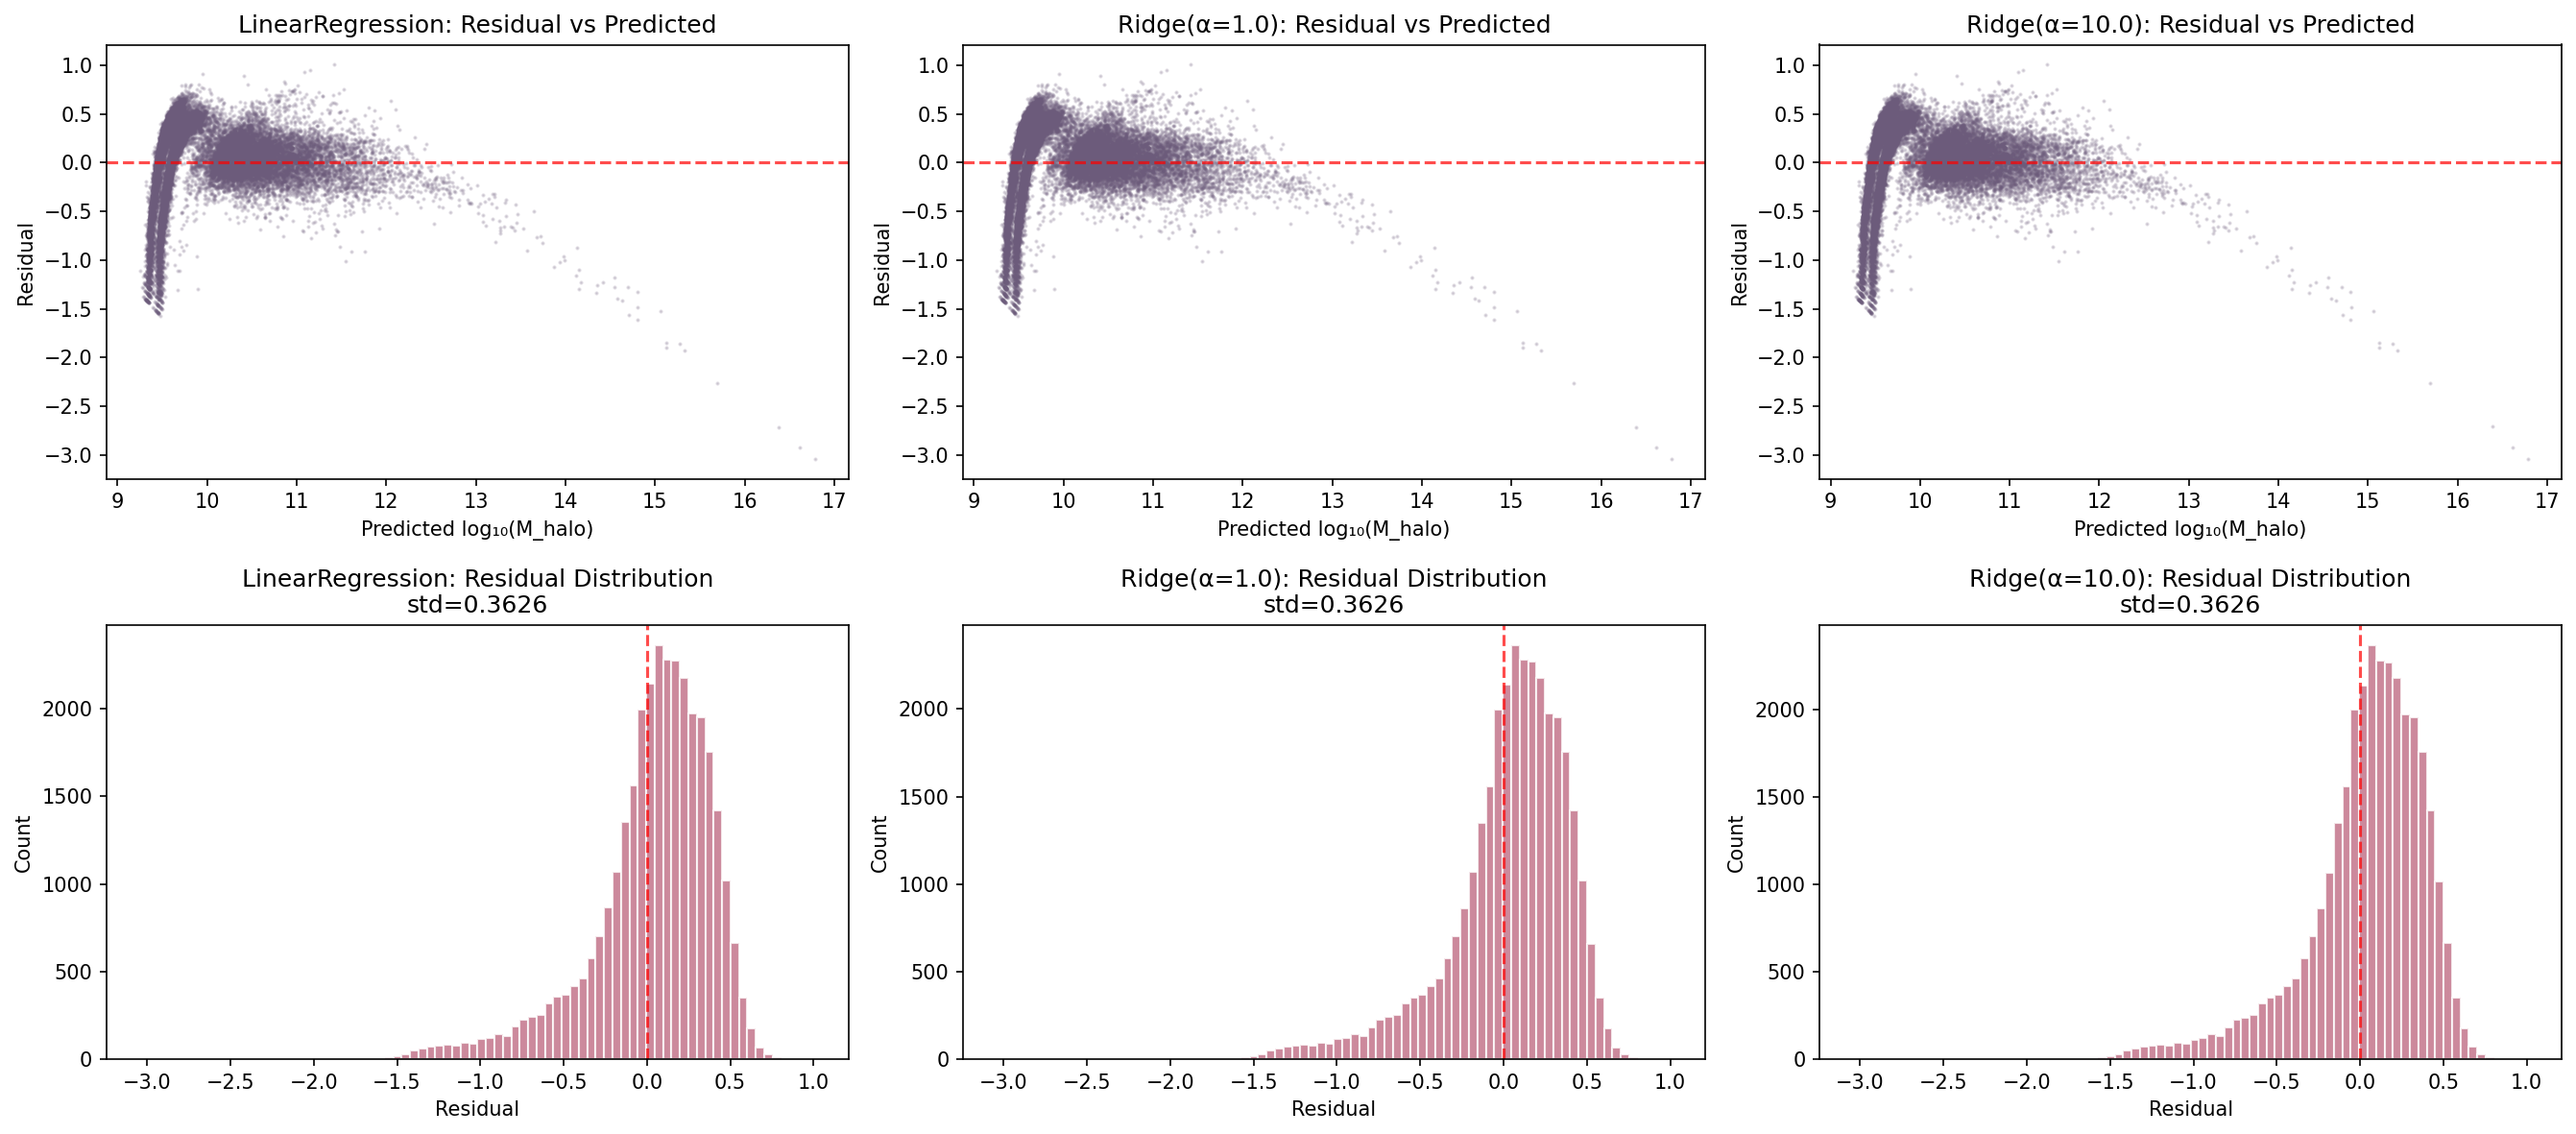
\includegraphics[width=0.85\textwidth]{step5_linear/residual_plot.png}
  \caption{Residuals ($\hat{y} - y$) for the linear model.  The residual histogram (right panel) shows mild positive excess kurtosis relative to a Gaussian, and the residual scatter (left panel) reveals structure at the mass extremes.}
  \label{fig:linear_resid}
\end{figure}


\subsection{Tree-Ensemble Models}
\label{sec:trees}

To capture the non-linear structure evident in the linear residuals, we train random forest (RF) and gradient-boosted tree (XGBoost) models.  Both are fitted on the same six log-transformed and raw features as the linear model, but \emph{without} standardization, since tree-based methods are invariant to monotonic feature transformations.

\subsubsection{Hyperparameter Selection}
\label{sec:tree_hp}

Model selection is performed via a grid search over three configurations per model family, evaluated on the validation set.  The configurations and their validation scores are reported in Table~\ref{tab:tree_hp}.

\begin{table}[H]
  \centering
  \caption{Hyperparameter configurations and validation-set performance for RF and XGBoost.  The best configuration (lowest validation RMSE) for each model family is indicated in bold.}
  \label{tab:tree_hp}
  \begin{tabular}{@{}lllcc@{}}
    \toprule
    Model & Config & & Val RMSE & Val $R^2$ \\
    \midrule
    \multirow{3}{*}{RF}
      & \textbf{$n = 200$, $d = 15$, $m_l = 5$}  && \textbf{0.0976} & \textbf{0.9792} \\
      & $n = 300$, $d = 20$, $m_l = 3$            && 0.0988 & 0.9787 \\
      & $n = 300$, $d = \infty$, $m_l = 2$        && 0.0996 & 0.9783 \\
    \midrule
    \multirow{3}{*}{XGBoost}
      & \textbf{$n = 300$, $d = 6$, $\eta = 0.1$} && \textbf{0.0977} & \textbf{0.9791} \\
      & $n = 500$, $d = 8$, $\eta = 0.05$         && 0.0984 & 0.9788 \\
      & $n = 500$, $d = 10$, $\eta = 0.05$        && 0.1000 & 0.9781 \\
    \bottomrule
  \end{tabular}
\end{table}

For RF, moderate depth ($d = 15$) with a minimum leaf size of 5 outperforms both the deeper and the fully grown variants, suggesting that slight regularization prevents overfitting to realization-specific noise.  For XGBoost, the most compact configuration ($d = 6$, $\eta = 0.1$, 300 trees) marginally outperforms deeper ensembles with halved learning rate, consistent with the bias--variance trade-off favouring simpler trees combined with a higher step size.

\subsubsection{Test-Set Evaluation}
\label{sec:tree_eval}

\begin{table}[H]
  \centering
  \caption{Best RF and XGBoost test-set performance compared to the Ridge baseline.  Tree models reduce RMSE by $\sim$71\% relative to the linear model.}
  \label{tab:tree_results}
  \begin{tabular}{@{}llccc@{}}
    \toprule
    Model & Split & RMSE & MAE & $R^2$ \\
    \midrule
    \multirow{3}{*}{Random Forest}
      & Train & 0.0846 & 0.0540 & 0.9867 \\
      & Val   & 0.0976 & 0.0633 & 0.9792 \\
      & Test  & 0.1042 & 0.0681 & 0.9798 \\
    \midrule
    \multirow{3}{*}{XGBoost}
      & Train & 0.0980 & 0.0639 & 0.9821 \\
      & Val   & 0.0977 & 0.0633 & 0.9791 \\
      & Test  & 0.1044 & 0.0680 & 0.9797 \\
    \midrule
    Ridge (baseline) & Test & 0.3640 & 0.2748 & 0.7537 \\
    \bottomrule
  \end{tabular}
\end{table}

Both tree models achieve test $R^2 \approx 0.980$, representing a dramatic improvement over the linear baseline ($R^2 = 0.754$).  The RMSE drops from 0.364~dex to $\sim$0.104~dex---a 71\% reduction, corresponding to a factor-of-3.5 improvement in typical prediction error.  RF and XGBoost are statistically indistinguishable on the test set ($\Delta R^2 \approx 0.0001$), though RF shows slightly larger train--test gap (train $R^2 = 0.987$ vs.\ test $R^2 = 0.980$), indicative of mild overfitting.

Diagnostic plots (Figures~\ref{fig:tree_pred} and~\ref{fig:tree_resid}) confirm that the tree models eliminate the systematic curvature seen in the linear residuals.  The predicted-vs-true scatter now tracks the identity line tightly across the full mass range.

\begin{figure}[H]
  \centering
  
\includegraphics[width=0.85\textwidth]{step6_trees/pred_vs_true.png}
  \caption{Predicted vs.\ true $\logMhalo$ for the best RF and XGBoost models.  Both track the identity line closely, with minimal scatter.}
  \label{fig:tree_pred}
\end{figure}

\begin{figure}[H]
  \centering
  
\includegraphics[width=0.85\textwidth]{step6_trees/residual_plot.png}
  \caption{Residual plots for RF and XGBoost.  Residuals are centred near zero with standard deviation $\sim$0.10~dex, and no systematic trend with mass is evident.}
  \label{fig:tree_resid}
\end{figure}


\subsubsection{SHAP Feature Importance}
\label{sec:shap}

To move beyond aggregate importance scores, we apply SHAP (SHapley Additive exPlanations) to the best random forest model.  SHAP values quantify each feature's contribution to individual predictions, grounded in cooperative game theory.  Table~\ref{tab:importance} compares the RF built-in (mean decrease in impurity) and SHAP (mean absolute SHAP value) importance rankings.

\begin{table}[H]
  \centering
  \caption{Feature importance: RF built-in impurity importance versus SHAP mean $|\phi_j|$.  Both methods agree on the ranking, with $\sigmav$ overwhelmingly dominant.}
  \label{tab:importance}
  \begin{tabular}{@{}lcc@{}}
    \toprule
    Feature & RF Importance & SHAP $\overline{|\phi_j|}$ \\
    \midrule
    $\sigmav$                         & 0.805 & 0.531 \\
    $\log_{10}(\Mstar + 1)$           & 0.166 & 0.085 \\
    $r_{1/2}$                         & 0.024 & 0.046 \\
    $\log_{10}(M_\mathrm{gas} + 1)$   & 0.003 & 0.013 \\
    $d_{5\mathrm{NN}}$                & 0.002 & 0.003 \\
    SFR                               & 0.000 & 0.001 \\
    \bottomrule
  \end{tabular}
\end{table}

Both methods agree on the ranking and confirm a strongly hierarchical importance structure.  Velocity dispersion accounts for 80.5\% of the RF impurity importance and contributes a mean $|\phi| = 0.531$~dex per prediction---more than six times the contribution of the second-ranked feature.  This is physically consistent: $\sigmav$ is a direct tracer of the halo's gravitational potential, whereas the remaining features encode secondary information about the galaxy's star formation history and baryon content.

Stellar mass ($\overline{|\phi|} = 0.085$) provides the strongest supplementary signal, reflecting the SHMR.  Half-mass radius ($\overline{|\phi|} = 0.046$) adds a modest geometric correction---at fixed $\sigmav$ and $\Mstar$, more extended galaxies tend to reside in slightly different halo environments.  Gas mass, environment distance, and star formation rate contribute marginally, suggesting that their information content is largely redundant given the other features.

The SHAP beeswarm plot (Figure~\ref{fig:shap}) provides additional insight into the directionality and functional form of each feature's contribution.

\begin{figure}[H]
  \centering
  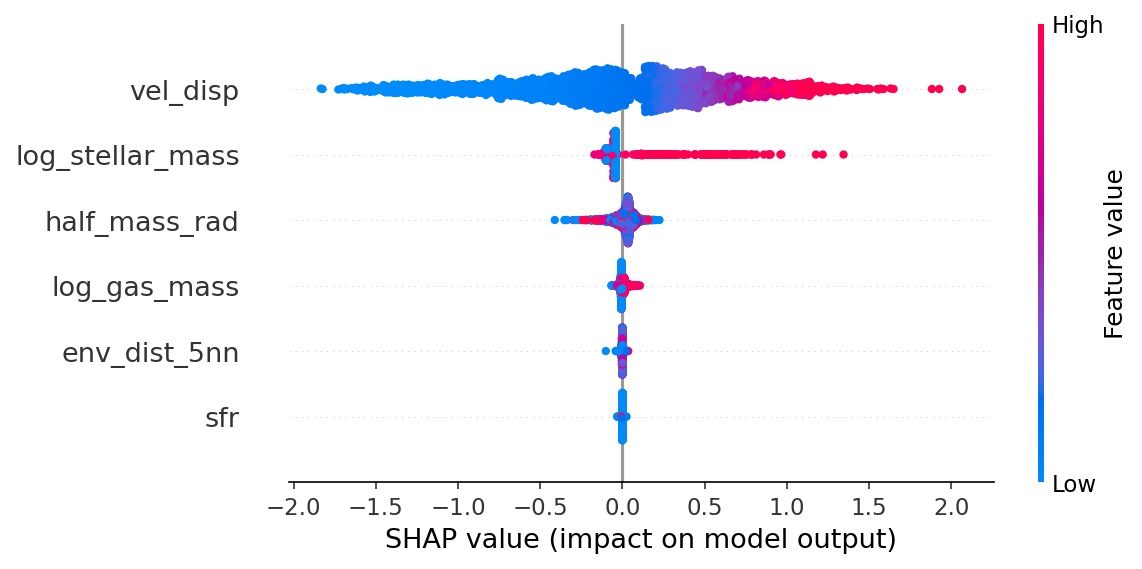
\includegraphics[width=0.80\textwidth]{step6_trees/shap_importance.png}
  \caption{SHAP beeswarm plot for the best RF model.  Each dot represents one prediction; horizontal position is the SHAP value ($\phi_j$), colour encodes the feature value (red = high, blue = low).  $\sigmav$ shows a wide, monotonic positive relationship: higher velocity dispersion consistently pushes the prediction to higher halo mass.}
  \label{fig:shap}
\end{figure}

% ~~~~~~~~~~~~~~~~~~~~~~~~~~~~~~~~~~~~~~~~~~~~~~~~~~~~~~~~~~~~~~~~~~~~~~~~~~~~
%  SECTION 5: MLP WITH MC DROPOUT
% ~~~~~~~~~~~~~~~~~~~~~~~~~~~~~~~~~~~~~~~~~~~~~~~~~~~~~~~~~~~~~~~~~~~~~~~~~~~~
\section{Neural Network with MC Dropout Uncertainty}
\label{sec:mlp}

Having established that tree-based models substantially outperform linear methods, we now evaluate whether a neural network can further improve prediction accuracy and, more importantly, whether it can provide calibrated uncertainty estimates via Monte Carlo Dropout.

\subsection{Architecture and Training}
\label{sec:mlp_arch}

We train a three-layer feed-forward multilayer perceptron (MLP) implemented in PyTorch.  The architecture is summarized in Table~\ref{tab:mlp_arch}.

\begin{table}[H]
  \centering
  \caption{MLP architecture and training configuration.  The network has \num{43905} learnable parameters.}
  \label{tab:mlp_arch}
  \begin{tabular}{@{}ll@{}}
    \toprule
    Component & Specification \\
    \midrule
    Input dimension   & 6 (log-transformed mass features + raw features) \\
    Hidden layers     & $256 \rightarrow 128 \rightarrow 64$ \\
    Activations       & ReLU after each hidden layer \\
    Normalization     & BatchNorm after each linear layer \\
    Regularization    & Dropout($p = 0.1$) after each activation \\
    Output            & 1 (linear, no activation) \\
    \midrule
    Loss function     & MSE (mean squared error) \\
    Optimizer         & Adam ($\eta = 10^{-3}$, weight decay $= 10^{-5}$) \\
    LR scheduler      & ReduceLROnPlateau (factor $= 0.5$, patience $= 10$) \\
    Batch size        & 1024 \\
    Max epochs        & 100 \\
    Early stopping    & Patience $= 20$ on validation loss \\
    \midrule
    Parameters        & \num{43905} \\
    Device            & CPU \\
    Training time     & 552.3\,s \\
    \bottomrule
  \end{tabular}
\end{table}

Features are preprocessed identically to the linear model: $\log_{10}(x + 1)$ applied to stellar mass and gas mass, followed by standardization (zero mean, unit variance) using statistics from the training set only.

Training proceeded for 89 of 100 scheduled epochs before early stopping was triggered.  The learning rate was reduced twice during training: from $10^{-3}$ to $5 \times 10^{-4}$ at approximately epoch~35, and to $2.5 \times 10^{-4}$ at epoch~65.  The best validation loss (0.0101) was achieved at epoch~69.  The training curve (Figure~\ref{fig:mlp_training}) shows a clear convergence pattern with no evidence of overfitting, as the validation loss tracks the training loss closely throughout.

\begin{figure}[H]
  \centering
  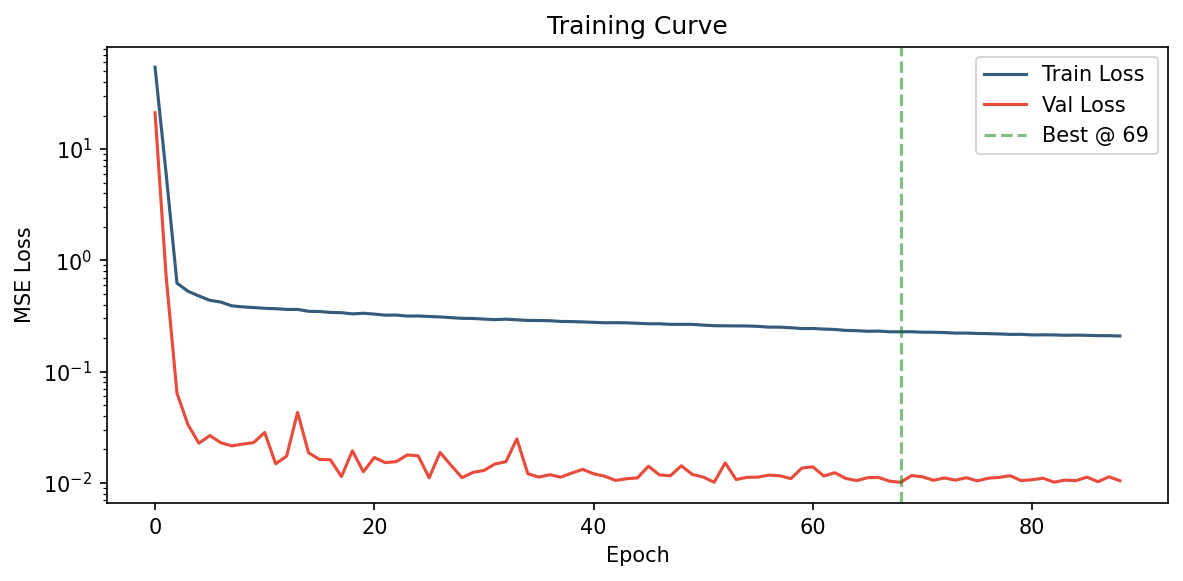
\includegraphics[width=0.80\textwidth]{step7_mlp/training_curve.png}
  \caption{MLP training and validation loss over 89 epochs.  Early stopping triggers at epoch~89 with the best model restored from epoch~69.  The learning rate schedule is visible as slope changes (epochs $\sim$35 and $\sim$65).}
  \label{fig:mlp_training}
\end{figure}


\subsection{Predictive Performance}
\label{sec:mlp_eval}

\begin{table}[H]
  \centering
  \caption{MLP test-set performance compared to the best tree models.}
  \label{tab:mlp_results}
  \begin{tabular}{@{}llccc@{}}
    \toprule
    Model & Split & RMSE & MAE & $R^2$ \\
    \midrule
    \multirow{3}{*}{MLP}
      & Train & 0.1109 & 0.0744 & 0.9771 \\
      & Val   & 0.1005 & 0.0681 & 0.9779 \\
      & Test  & 0.1079 & 0.0733 & 0.9784 \\
    \midrule
    RF (reference) & Test & 0.1042 & 0.0681 & 0.9798 \\
    \bottomrule
  \end{tabular}
\end{table}

The MLP achieves test $R^2 = 0.9784$ with RMSE $= 0.1079$~dex (Table~\ref{tab:mlp_results}).  This is competitive with, but marginally below, the tree ensembles ($R^2 = 0.9798$, RMSE $= 0.1042$~dex for RF).  The gap ($\Delta R^2 = 0.0014$, $\Delta\text{RMSE} = 0.004$~dex) is small  but consistent across runs, and is in line with the broader finding in the tabular ML literature that tree-based methods tend to match or outperform neural networks on structured tabular data with moderate dimensionality.

Notably, the MLP shows minimal overfitting: the train--test $R^2$ gap is only 0.0013 (compared to 0.0069 for RF), suggesting that the combination of BatchNorm, Dropout, and weight decay provides effective regularization.

Predicted-vs-true and residual plots (Figures~\ref{fig:mlp_pred} and~\ref{fig:mlp_resid}) confirm that the MLP predictions follow the identity line closely and produce symmetric, zero-centred residuals without mass-dependent bias.

\begin{figure}[H]
  \centering
  
\includegraphics[width=0.80\textwidth]{step7_mlp/pred_vs_true.png}
  \caption{Predicted vs.\ true $\logMhalo$ for the MLP model on the test set.  The scatter closely follows the identity line.}
  \label{fig:mlp_pred}
\end{figure}

\begin{figure}[H]
  \centering
  
\includegraphics[width=0.80\textwidth]{step7_mlp/residual_plot.png}
  \caption{MLP residuals ($\hat{y} - y$) on the test set.  The residual distribution is approximately Gaussian with $\sigma \approx 0.108$~dex.}
  \label{fig:mlp_resid}
\end{figure}


\subsection{MC Dropout Uncertainty Quantification}
\label{sec:mcdropout}

A key advantage of the MLP architecture is the ability to produce calibrated predictive uncertainties via Monte Carlo (MC) Dropout.  At inference time, instead of disabling dropout (the standard \texttt{model.eval()} mode), we retain dropout in its active state (\texttt{model.train()}) and perform $T = 50$ stochastic forward passes for each test-set input.  Each pass applies a different random dropout mask, yielding a distribution of predictions from which we extract:

\begin{align}
  \hat{y}_\mathrm{mean} &= \frac{1}{T} \sum_{t=1}^{T} \hat{y}^{(t)}, &
  \hat{\sigma}_\mathrm{pred} &= \sqrt{\frac{1}{T-1} \sum_{t=1}^{T} \bigl(\hat{y}^{(t)} - \hat{y}_\mathrm{mean}\bigr)^2}.
\end{align}

The per-sample uncertainty $\hat{\sigma}_\mathrm{pred}$ quantifies the model's epistemic uncertainty---the component of prediction error attributable to model parameter uncertainty rather than irreducible noise.

\begin{table}[H]
  \centering
  \caption{MC Dropout uncertainty statistics on the test set ($T = 50$ forward passes).}
  \label{tab:mc_dropout}
  \begin{tabular}{@{}lr@{}}
    \toprule
    Statistic & Value [dex] \\
    \midrule
    Mean $\hat{\sigma}_\mathrm{pred}$     & 0.452 \\
    Median $\hat{\sigma}_\mathrm{pred}$   & 0.449 \\
    90th percentile $\hat{\sigma}_\mathrm{pred}$ & 0.528 \\
    \bottomrule
  \end{tabular}
\end{table}

The mean predictive uncertainty is 0.452~dex (Table~\ref{tab:mc_dropout}), which is roughly four times the actual RMSE of 0.108~dex.  This overestimation is a known property of MC Dropout uncertainty: because only a small fraction of parameters are randomized per pass (dropout rate $p = 0.1$), the variance of the resulting predictions reflects the sensitivity of the output to individual neurons rather than the true posterior width.  The uncertainty is therefore better interpreted as a \emph{relative} measure of confidence---predictions with higher $\hat{\sigma}$ are genuinely less reliable---rather than a calibrated absolute error bar.

Figure~\ref{fig:uncertainty} visualizes the relationship between predicted mass, actual error, and MC Dropout uncertainty.

\begin{figure}[H]
  \centering
  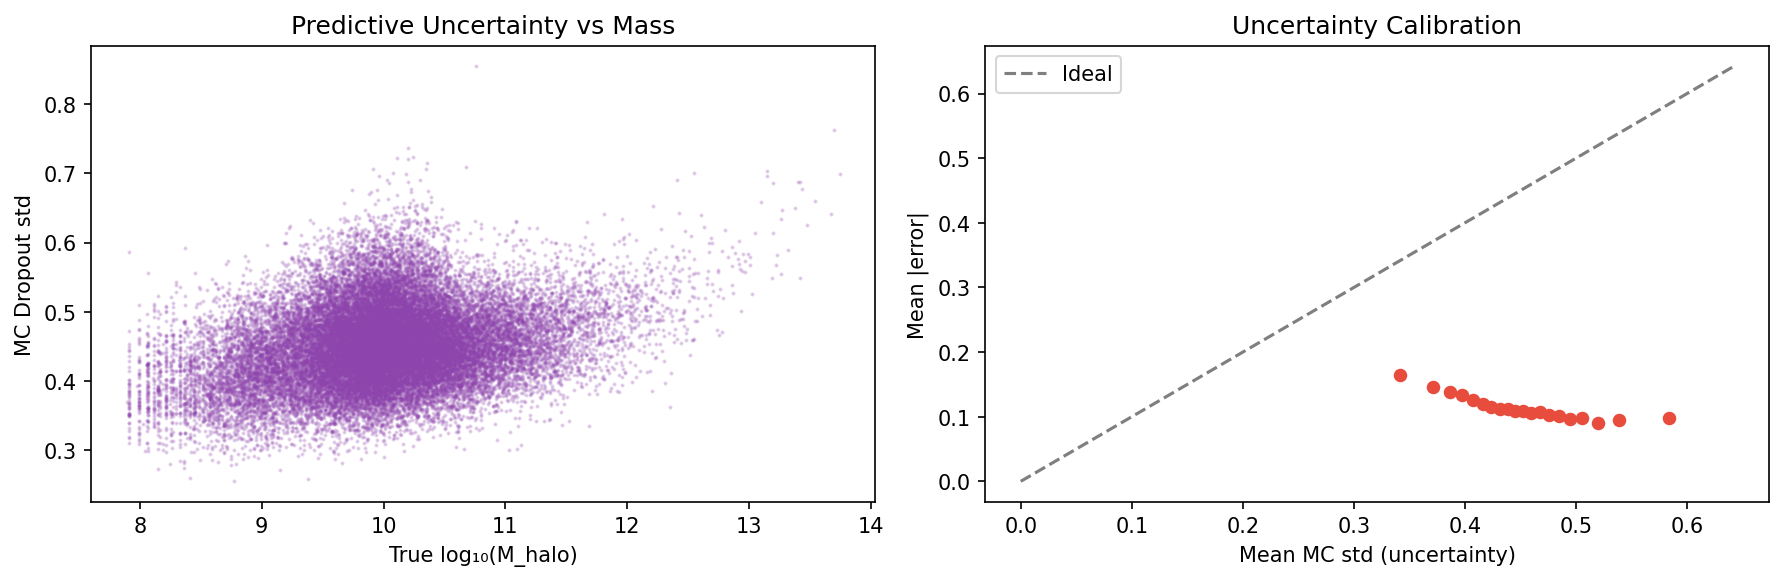
\includegraphics[width=0.85\textwidth]{step7_mlp/uncertainty_plot.png}
  \caption{MC Dropout uncertainty analysis.  Top: scatter of predictions coloured by uncertainty.  Bottom: binned comparison of mean $\hat{\sigma}_\mathrm{pred}$ against mean absolute error, showing positive (though imperfect) correlation.}
  \label{fig:uncertainty}
\end{figure}


% ~~~~~~~~~~~~~~~~~~~~~~~~~~~~~~~~~~~~~~~~~~~~~~~~~~~~~~~~~~~~~~~~~~~~~~~~~~~~
%  SECTION 6: UNIFIED EVALUATION & ANALYSIS
% ~~~~~~~~~~~~~~~~~~~~~~~~~~~~~~~~~~~~~~~~~~~~~~~~~~~~~~~~~~~~~~~~~~~~~~~~~~~~
\section{Unified Evaluation and Analysis}
\label{sec:unified}

This section consolidates results across all four model classes and presents targeted diagnostic analyses: a unified comparison table, mass-binned error decomposition, data scaling laws, and feature importance comparison.

\subsection{Model Comparison}
\label{sec:comparison}

Table~\ref{tab:unified} summarizes the performance of all four models across the three data splits.

\begin{table}[H]
  \centering
  \caption{Unified model comparison across all splits.  Models are ordered by increasing test $R^2$.  Bold indicates the best test-set value per metric.}
  \label{tab:unified}
  \begin{tabular}{@{}llccc@{}}
    \toprule
    Model & Split & RMSE [dex] & MAE [dex] & $R^2$ \\
    \midrule
    \multirow{3}{*}{Ridge}
      & Train & 0.3554 & 0.2628 & 0.7648 \\
      & Val   & 0.3034 & 0.2309 & 0.7988 \\
      & Test  & 0.3640 & 0.2748 & 0.7537 \\
    \midrule
    \multirow{3}{*}{MLP}
      & Train & 0.1109 & 0.0744 & 0.9771 \\
      & Val   & 0.1005 & 0.0681 & 0.9779 \\
      & Test  & 0.1079 & 0.0733 & 0.9784 \\
    \midrule
    \multirow{3}{*}{XGBoost}
      & Train & 0.0980 & 0.0639 & 0.9821 \\
      & Val   & 0.0977 & 0.0633 & 0.9791 \\
      & Test  & 0.1044 & 0.0680 & 0.9797 \\
    \midrule
    \multirow{3}{*}{\textbf{Random Forest}}
      & Train & 0.0846 & 0.0540 & 0.9867 \\
      & Val   & 0.0976 & 0.0633 & 0.9792 \\
      & Test  & \textbf{0.1042} & \textbf{0.0681} & \textbf{0.9798} \\
    \bottomrule
  \end{tabular}
\end{table}

Three key observations emerge:

\begin{enumerate}[nosep]
  \item \textbf{Non-linearity is critical.}  The jump from Ridge ($R^2 = 0.754$) to RF ($R^2 = 0.980$) amounts to a 30\% increase in explained variance and a 71\% reduction in RMSE.  This confirms that the mapping from baryonic features to halo mass contains substantial non-linear structure that linear methods cannot capture.
  
  \item \textbf{Trees match or exceed neural networks.}  RF and XGBoost are statistically indistinguishable ($\Delta R^2 = 0.0001$), and both marginally outperform the MLP ($\Delta R^2 = 0.0014$).  This is consistent with the growing consensus that gradient-boosted trees and random forests remain competitive with, and often superior to, neural networks on tabular data of moderate dimensionality.
  
  \item \textbf{Overfitting is well controlled.}  The largest train--test $R^2$ gap is 0.0069 (RF), while the MLP gap is only 0.0013.  No model shows catastrophic overfitting, validating the regularization strategies employed.
\end{enumerate}

Figure~\ref{fig:combined_pred} overlays the predicted-vs-true scatter for all four models, providing a visual summary of the performance hierarchy.

\begin{figure}[H]
  \centering
  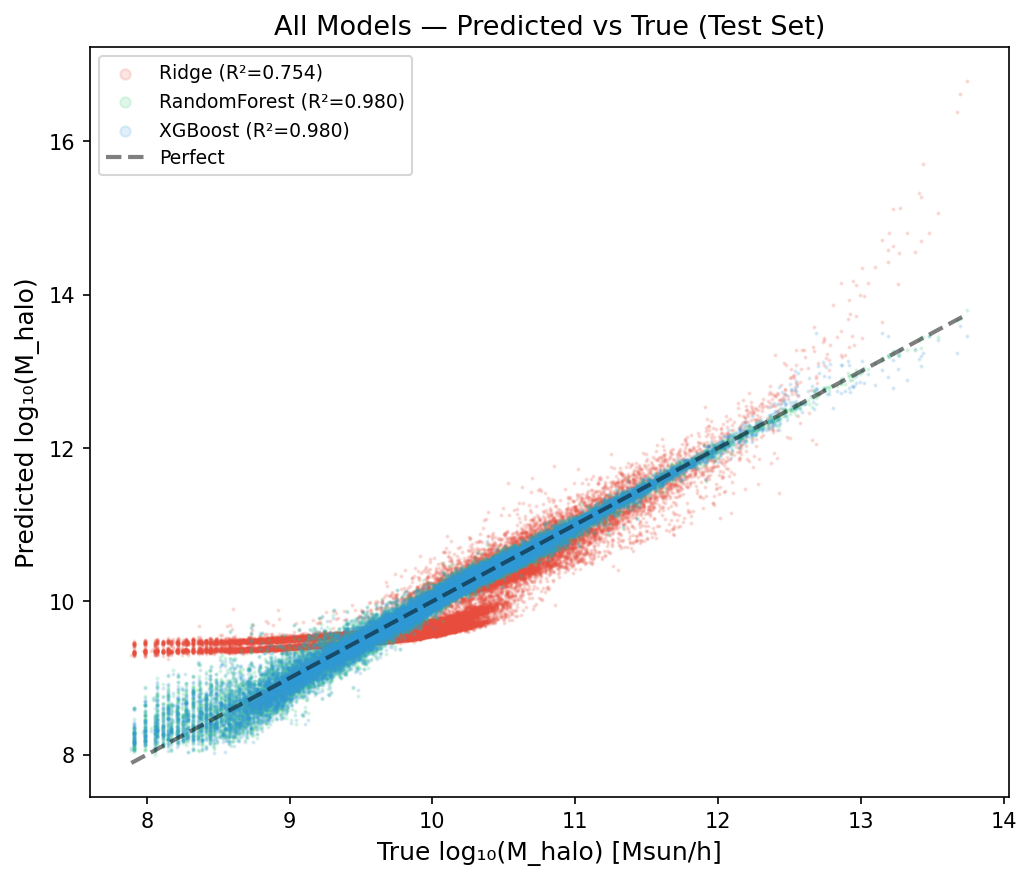
\includegraphics[width=0.95\textwidth]{step8_final/combined_pred_vs_true.png}
  \caption{Predicted vs.\ true $\logMhalo$ for all four models (test set).  Ridge shows clear curvature at the extremes; the three non-linear models collapse onto the identity line.}
  \label{fig:combined_pred}
\end{figure}


\subsection{Mass-Binned Error Analysis}
\label{sec:massbins}

To identify mass regimes where models struggle, we partition the test set into seven bins by true $\logMhalo$ and compute per-bin RMSE and MAE.  Table~\ref{tab:mass_bins} reports the results.

\begin{table}[H]
  \centering
  \caption{Mass-binned RMSE on the test set.  Counts reflect the number of halos per bin.  The lowest RMSE per bin is shown in bold.}
  \label{tab:mass_bins}
  \begin{tabular}{@{}lrcccc@{}}
    \toprule
    Mass bin & Count & Ridge & RF & XGBoost \\
    \midrule
    $[7.5, 9.0)$    & \num{2954}  & 0.840 & \textbf{0.244} & 0.245 \\
    $[9.0, 10.0)$   & \num{13750} & 0.240 & 0.092 & \textbf{0.091} \\
    $[10.0, 10.5)$  & \num{9319}  & 0.329 & 0.064 & \textbf{0.062} \\
    $[10.5, 11.0)$  & \num{4072}  & 0.227 & 0.069 & \textbf{0.068} \\
    $[11.0, 11.5)$  & \num{1739}  & 0.233 & 0.057 & \textbf{0.056} \\
    $[11.5, 12.0)$  & 623         & 0.266 & 0.049 & \textbf{0.048} \\
    $[12.0, 15.0)$  & 310         & 0.600 & \textbf{0.042} & 0.135 \\
    \bottomrule
  \end{tabular}
\end{table}

Several patterns are physically informative:

\paragraph{Low-mass regime $[\mathbf{7.5, 9.0})$.}
This is the most challenging bin for all models.  Ridge RMSE peaks at 0.840~dex---nearly an order of magnitude in mass---reflecting the extreme non-linearity of the $\sigmav$--$M$ relation for dwarf-scale halos.  Even RF achieves only 0.244~dex, which is $\sim$2.4$\times$ its global average.  These halos are intrinsically noisy: their baryonic content is dominated by stochastic processes (reionisation, feedback), and velocity dispersion measurements are based on few particles.

\paragraph{Mid-mass regime $[\mathbf{9.0, 12.0})$.}
RF and XGBoost are tightly matched, with RMSE ranging from 0.048 to 0.092~dex.  This regime contains the bulk of the data (29,503 of 32,767 test halos, 90\%) and encompasses the ``sweet spot'' where both the virial-theorem and SHMR signals are strongest and best resolved.

\paragraph{Cluster-scale regime $[\mathbf{12.0, 15.0})$.}
RF (RMSE $= 0.042$~dex) dramatically outperforms XGBoost (RMSE $= 0.135$~dex) in this rare, high-mass bin ($n = 310$).  The XGBoost degradation may stem from its boosting strategy: with only 310 cluster-scale halos in the test set, the model has limited exposure to this regime during training, and the sequential correction mechanism of gradient boosting may over-regularise at the distribution tails.  RF's bagging approach, by contrast, naturally includes these extreme samples in individual trees.

Figure~\ref{fig:mass_bins} visualises the per-bin RMSE and MAE comparison.

\begin{figure}[H]
  \centering
  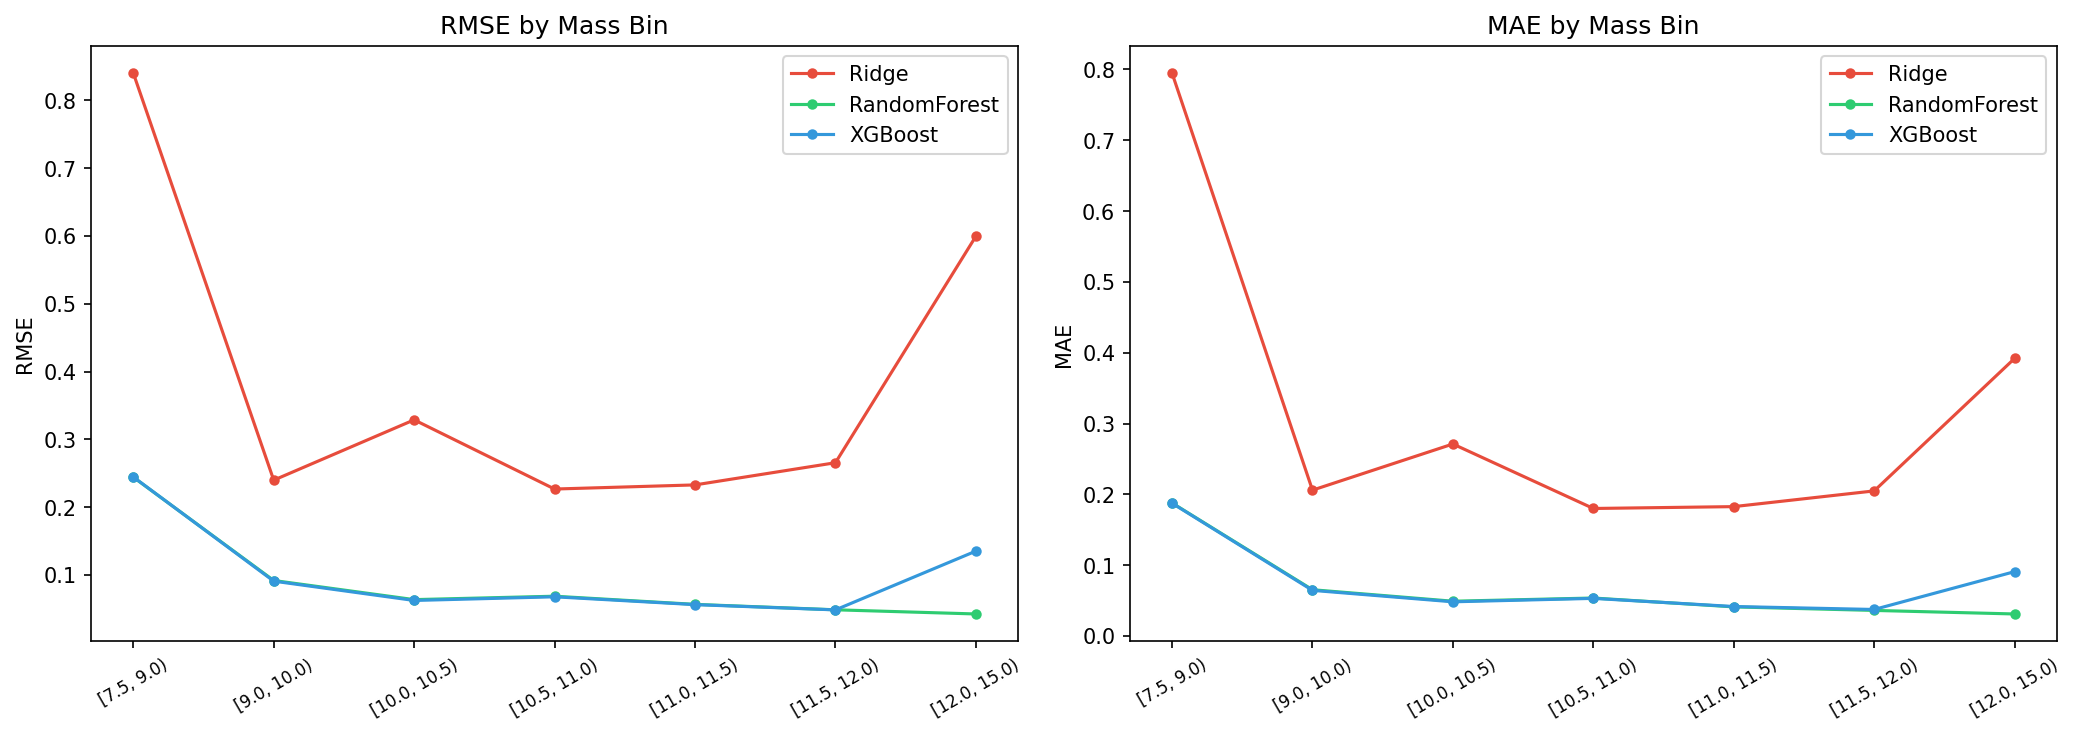
\includegraphics[width=0.90\textwidth]{step8_final/mass_binned_errors.png}
  \caption{Mass-binned RMSE and MAE for Ridge, RF, and XGBoost.  Error is highest at the mass extremes (low-mass dwarfs and cluster-scale halos) and lowest in the intermediate regime $[10, 12)$~dex.}
  \label{fig:mass_bins}
\end{figure}


\subsection{Data Scaling Analysis}
\label{sec:scaling}

To assess sample efficiency and diagnose whether additional training data would improve performance, we train Ridge and RF models on progressively larger subsets of the training set (5\%, 10\%, 25\%, 50\%, 75\%, 100\%) and evaluate on the full test set.  Table~\ref{tab:scaling} and Figure~\ref{fig:scaling} report the results.

\begin{table}[H]
  \centering
  \caption{Data scaling: test-set RMSE and $R^2$ as a function of training set fraction.}
  \label{tab:scaling}
  \begin{tabular}{@{}rr|cc|cc@{}}
    \toprule
    Fraction & $n_\mathrm{train}$ & Ridge RMSE & Ridge $R^2$ & RF RMSE & RF $R^2$ \\
    \midrule
    5\%   & \num{7957}   & 0.367 & 0.750 & 0.109 & 0.978 \\
    10\%  & \num{15914}  & 0.366 & 0.751 & 0.107 & 0.979 \\
    25\%  & \num{39785}  & 0.365 & 0.753 & 0.106 & 0.979 \\
    50\%  & \num{79571}  & 0.365 & 0.753 & 0.105 & 0.979 \\
    75\%  & \num{119357} & 0.365 & 0.753 & 0.105 & 0.980 \\
    100\% & \num{159143} & 0.364 & 0.754 & 0.104 & 0.980 \\
    \bottomrule
  \end{tabular}
\end{table}

Two striking conclusions emerge:

\paragraph{RF is remarkably sample-efficient.}
With only 5\% of the training data ($n = \num{7957}$), RF already achieves $R^2 = 0.978$ and RMSE $= 0.109$~dex---within 0.005~dex of its full-data performance.  Increasing from 5\% to 100\% reduces RMSE by merely 0.005~dex ($<$5\% relative improvement).  This plateau indicates that the signal in the $\sigmav$--$\Mhalo$ mapping is so strong that a relatively small number of examples suffices to learn it to near-optimal accuracy.

\paragraph{Ridge is data-saturated.}
Ridge performance is essentially flat across all fractions ($\Delta R^2 < 0.004$ from 5\% to 100\%).  The linear model captures the leading-order correlations immediately and cannot benefit from additional data because the remaining variance is non-linear in nature.  This confirms that the performance ceiling of linear models on this task is approximately $R^2 \approx 0.75$, determined by the functional form of the model class rather than by data insufficiency.

\begin{figure}[H]
  \centering
  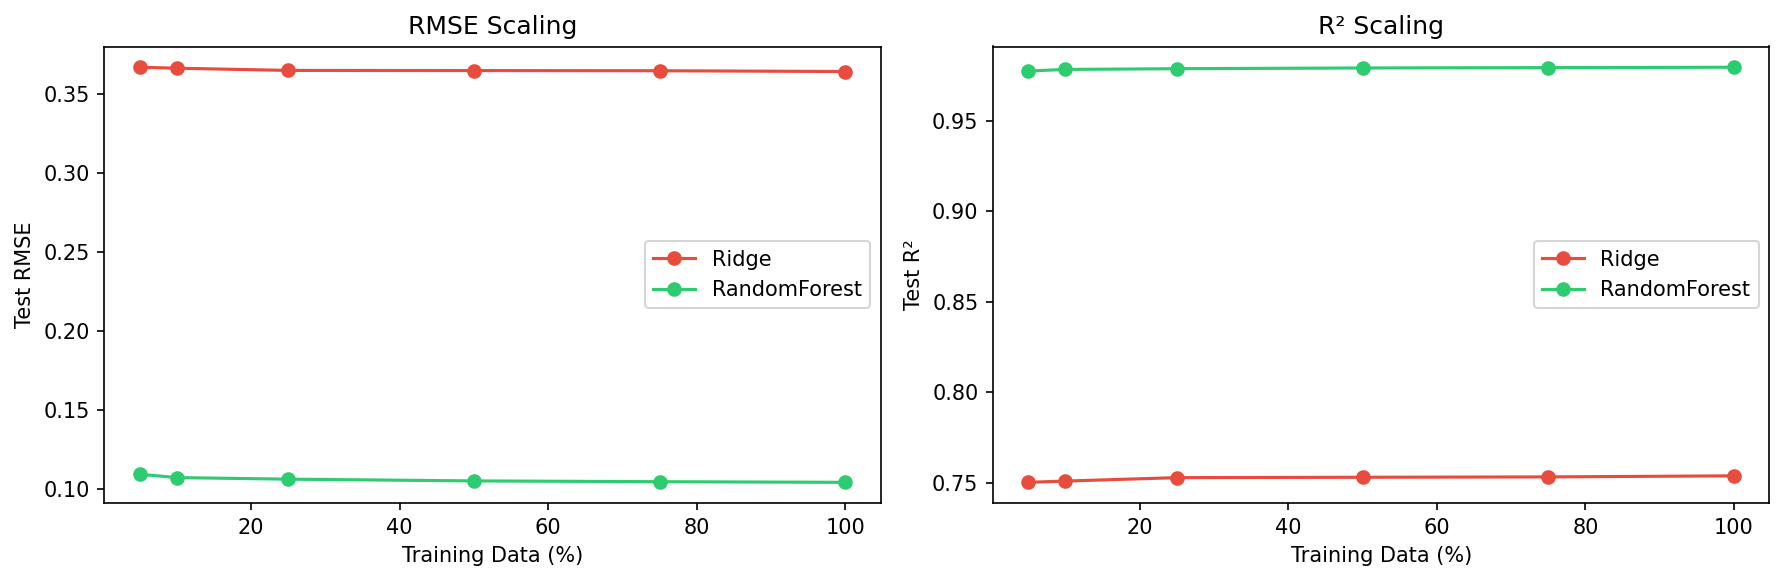
\includegraphics[width=0.85\textwidth]{step8_final/data_scaling.png}
  \caption{Data scaling curves for Ridge and RF.  RF reaches near-asymptotic performance with $\sim$5\% of the training data; Ridge is flat across all fractions.}
  \label{fig:scaling}
\end{figure}


\subsection{Feature Importance Comparison}
\label{sec:feat_comparison}

To assess whether linear and non-linear models rely on the same features, Figure~\ref{fig:feat_comparison} compares the normalised absolute coefficients from Ridge regression against the RF built-in (impurity-based) importances.

\begin{table}[H]
  \centering
  \caption{Normalised feature importance: Ridge (absolute standardized coefficients, normalised to sum to 1) versus RF (impurity-based importance).}
  \label{tab:feat_comparison}
  \begin{tabular}{@{}lcc@{}}
    \toprule
    Feature & Ridge (norm.) & RF (impurity) \\
    \midrule
    $\sigmav$                         & 0.623 & 0.805 \\
    $\log_{10}(\Mstar + 1)$           & 0.214 & 0.166 \\
    $\log_{10}(M_\mathrm{gas} + 1)$   & 0.080 & 0.003 \\
    $r_{1/2}$                         & 0.055 & 0.024 \\
    SFR                               & 0.023 & 0.000 \\
    $d_{5\mathrm{NN}}$                & 0.006 & 0.002 \\
    \bottomrule
  \end{tabular}
\end{table}

Both methods agree that $\sigmav$ is the dominant predictor and $\Mstar$ is second.  However, they diverge on gas mass and SFR: Ridge assigns 8.0\% and 2.3\% of total importance to these features, while RF assigns near-zero (0.3\% and 0.03\%, respectively).  This discrepancy arises because linear models treat gas mass and SFR as independent signals, whereas tree-based models can represent their contribution as interaction effects with $\sigmav$, rendering them redundant as standalone splits.

\begin{figure}[H]
  \centering
  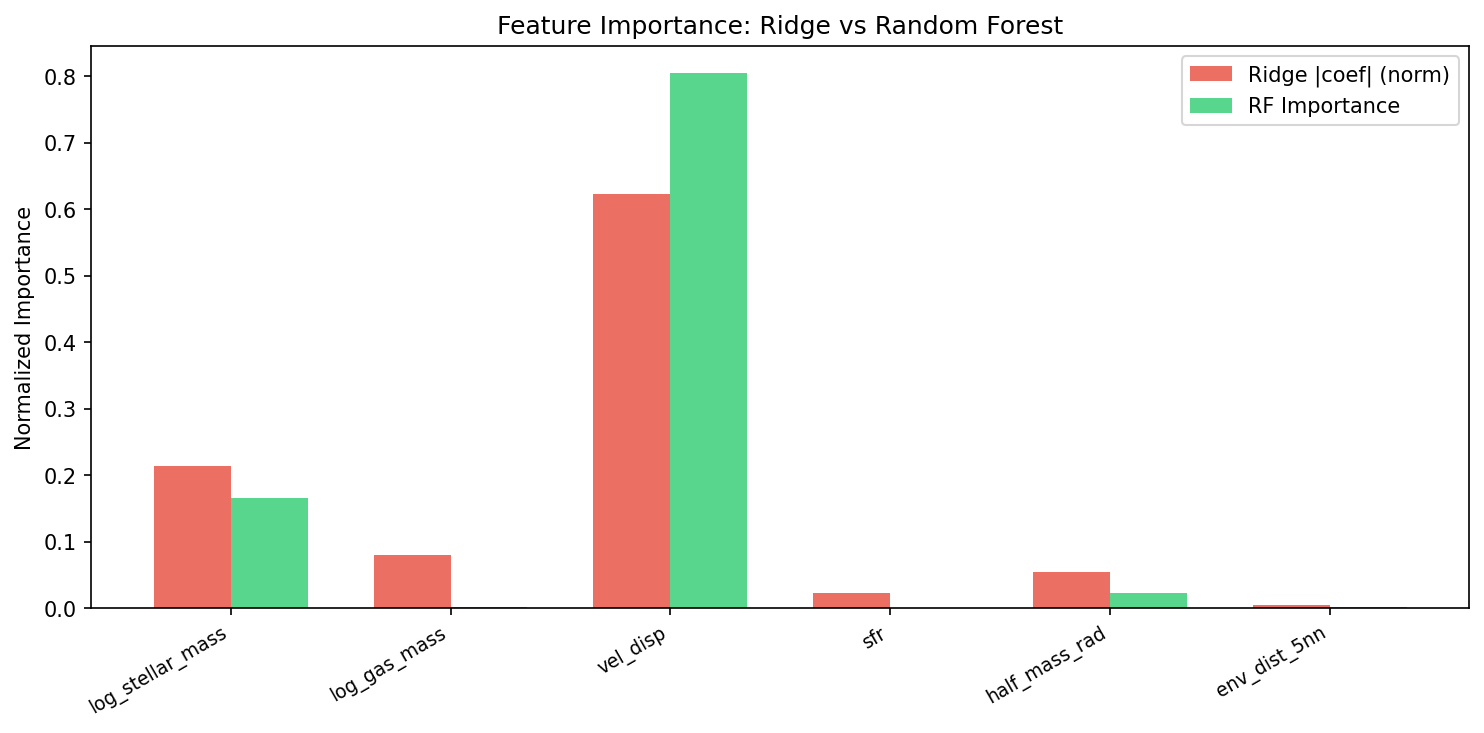
\includegraphics[width=0.85\textwidth]{step8_final/feature_importance_comparison.png}
  \caption{Side-by-side comparison of normalised feature importance for Ridge (absolute coefficient) and RF (impurity-based).  Both models agree on $\sigmav$ dominance; Ridge overweights gas mass and SFR relative to RF.}
  \label{fig:feat_comparison}
\end{figure}

% ~~~~~~~~~~~~~~~~~~~~~~~~~~~~~~~~~~~~~~~~~~~~~~~~~~~~~~~~~~~~~~~~~~~~~~~~~~~~
%  SECTION 7: SYMBOLIC REGRESSION
% ~~~~~~~~~~~~~~~~~~~~~~~~~~~~~~~~~~~~~~~~~~~~~~~~~~~~~~~~~~~~~~~~~~~~~~~~~~~~
\section{Symbolic Regression}
\label{sec:pysr}

While tree-based and neural network models achieve high predictive accuracy, they function as black-box mappings.  In this section, we use PySR---a symbolic regression package based on evolutionary search---to discover compact, human-readable analytic formulas that approximate the $\logMhalo$ prediction task.  Such formulas, if sufficiently accurate, offer direct physical interpretability and are trivially deployable without machine learning infrastructure.

\subsection{Setup}
\label{sec:pysr_setup}

We provide PySR with the three features identified as most important by the SHAP analysis of Section~\ref{sec:shap}:

\begin{itemize}[nosep]
  \item $x_0 = \sigmav$ \quad (velocity dispersion, km/s)
  \item $x_1 = \log_{10}(\Mstar + 1)$ \quad (log stellar mass)
  \item $x_2 = r_{1/2}$ \quad (half-mass radius, kpc/$h$)
\end{itemize}

The search is configured with 40 iterations on a 10,000-row training subsample (random seed 42), using the operator set $\{+, -, \times, \div, \log, \sqrt{\cdot}, (\cdot)^2\}$.  PySR maintains a Pareto front of equations, trading model complexity (number of operators and operands) against MSE loss.

\subsection{Pareto Front of Discovered Equations}
\label{sec:pareto}

Table~\ref{tab:pareto} presents a selected subset of the Pareto front, ordered by complexity.  The full set of 12 equations is given in Appendix~\ref{app:pareto}.

\begin{table}[H]
  \centering
  \caption{Selected equations from the PySR Pareto front.  Complexity counts the total number of nodes in the expression tree.  Loss is the mean squared error on the training subsample.  The ``best'' equation (complexity~12) combines a logarithmic velocity dispersion term with a square-root radius correction.}
  \label{tab:pareto}
  \begin{tabular}{@{}rrl@{}}
    \toprule
    Complexity & Loss & Equation \\
    \midrule
    1  & 0.5429 & $\hat{y} = 9.986$ \quad (constant = $\overline{\logMhalo}$) \\[3pt]
    4  & 0.0447 & $\hat{y} = \ln(\sigmav) + 6.948$ \\[3pt]
    6  & 0.0425 & $\hat{y} = \ln(\sigmav - 1.281) + 7.027$ \\[3pt]
    8  & 0.0368 & $\hat{y} = 0.816\,\ln(\sigmav - 3.843) + 7.732$ \\[3pt]
    11 & 0.0338 & $\hat{y} = \ln(\sigmav - 1.657) + 7.380 - \dfrac{1.508}{\sqrt{r_{1/2}}}$ \\[6pt]
    \textbf{12} & \textbf{0.0293} & $\hat{y} = 0.833\,\ln(\sigmav - 3.644) + \sqrt{\sqrt{r_{1/2}} + 53.85}$ \\[3pt]
    17 & 0.0264 & $\hat{y} = 0.804\,\ln(\sigmav - 4.191) + \sqrt{\ln\bigl((r_{1/2} + 4.989 - x_1)^2\bigr) + 54.50}$ \\
    \bottomrule
  \end{tabular}
\end{table}


\subsection{Physical Interpretation}
\label{sec:pysr_interp}

The Pareto front reveals a clear hierarchy of physical effects:

\paragraph{Leading term: $\ln(\sigmav)$.}
The simplest useful equation (complexity~4) is $\hat{y} = \ln(\sigmav) + 6.95$, which alone achieves a loss of 0.045.  This is a direct expression of the virial theorem: for a virialized system, $M \propto \sigmav^2 R$, so $\log_{10} M \sim 2\log_{10}\sigmav + \text{const}$.  The natural logarithm ($\ln = \log_e$) differs from $\log_{10}$ only by a multiplicative constant ($\log_{10} x = \ln x / \ln 10 \approx 0.434\,\ln x$), so the discovered formula is dimensionally and functionally consistent with the virial scaling.

\paragraph{Threshold correction: $\ln(\sigmav - c)$.}
At complexity~6--8, PySR discovers that subtracting a constant from $\sigmav$ before taking the logarithm materially improves the fit (loss 0.045~$\rightarrow$~0.037).  Physically, this offset ($c \approx 3.6$--$4.1$~km/s) may represent a minimum velocity dispersion floor below which the virial scaling breaks down---indeed, the smallest $\sigmav$ in the dataset is 3.80~km/s.

\paragraph{Radius correction: $\sqrt{\sqrt{r_{1/2}} + \text{const}}$.}
The best equation (complexity~12) adds a term $\sqrt{\sqrt{r_{1/2}} + 53.85}$, which provides a weak, monotonically increasing correction indexed by galaxy size.  This is consistent with the virial relation $M \propto \sigmav^2 R$: at fixed $\sigmav$, a more spatially extended galaxy implies a larger halo virial radius and hence a higher enclosed mass.

\paragraph{Stellar mass appears only at high complexity.}
$x_1 = \log_{10}(\Mstar + 1)$ first enters the Pareto front at complexity~17, suggesting that its information content is largely redundant with $\sigmav$ and $r_{1/2}$ in the context of compact analytic formulas.


\subsection{Test-Set Accuracy}
\label{sec:pysr_test}

The best equation (complexity~12) is evaluated on the full test set (\num{32767} halos):

\begin{table}[H]
  \centering
  \caption{PySR best equation test-set performance compared to the full ML models.}
  \label{tab:pysr_test}
  \begin{tabular}{@{}lccc@{}}
    \toprule
    Model & Test RMSE [dex] & Test $R^2$ & Parameters \\
    \midrule
    PySR (complexity 12) & 0.162 & 0.951 & 5 constants \\
    Ridge                & 0.364 & 0.754 & 6 coefficients \\
    RF                   & 0.104 & 0.980 & $\sim$10$^5$ splits \\
    MLP                  & 0.108 & 0.978 & \num{43905} weights \\
    \bottomrule
  \end{tabular}
\end{table}

The PySR formula captures 95.1\% of the target variance using only two features ($\sigmav$ and $r_{1/2}$) and five fitted constants---a remarkable compression relative to the $\sim$\num{43905}-parameter MLP.  The $R^2$ gap to RF ($\Delta R^2 = 0.029$) quantifies the cost of interpretability: a 3-percentage-point sacrifice in accuracy yields a formula that can be written on a single line and evaluated without any ML infrastructure.

\begin{figure}[H]
  \centering
  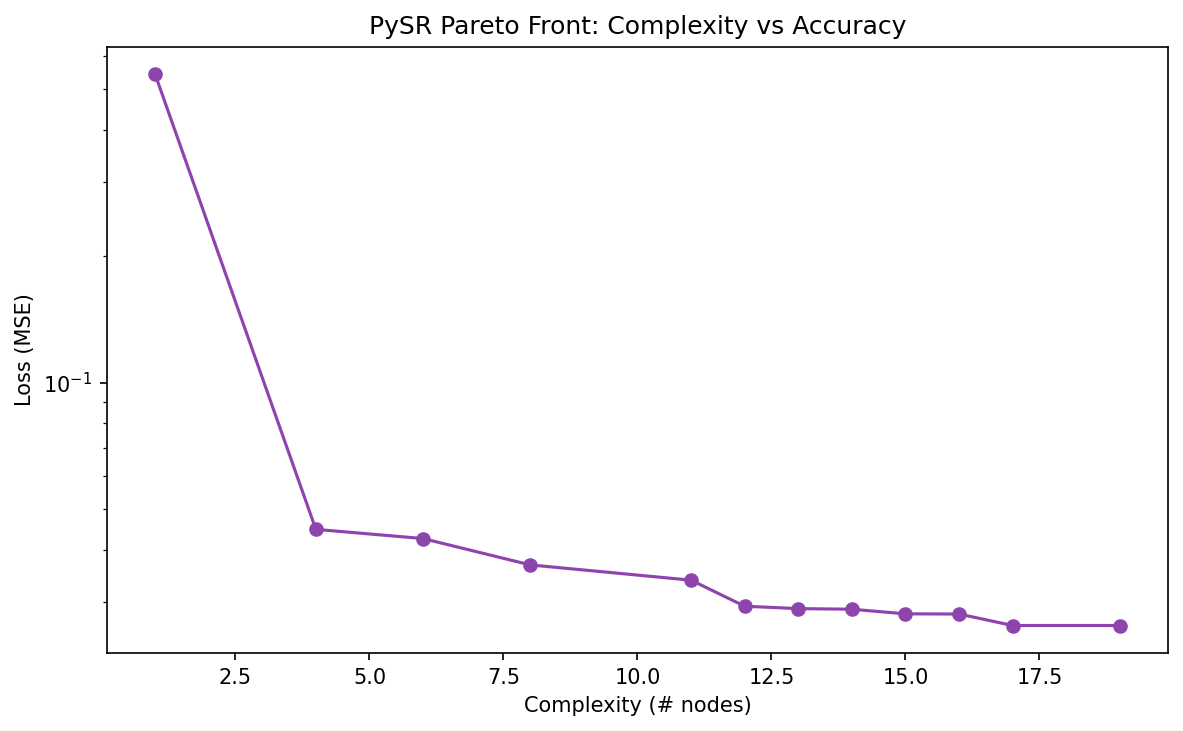
\includegraphics[width=0.80\textwidth]{step8_final/pysr_pareto.png}
  \caption{PySR Pareto front: equation complexity vs.\ loss.  The steepest improvement occurs at complexity~4 (addition of $\ln\sigmav$); the best complexity--accuracy trade-off is at complexity~12.}
  \label{fig:pareto}
\end{figure}


% ~~~~~~~~~~~~~~~~~~~~~~~~~~~~~~~~~~~~~~~~~~~~~~~~~~~~~~~~~~~~~~~~~~~~~~~~~~~~
%  SECTION 8: CROSS-SIMULATION TRANSFER
% ~~~~~~~~~~~~~~~~~~~~~~~~~~~~~~~~~~~~~~~~~~~~~~~~~~~~~~~~~~~~~~~~~~~~~~~~~~~~
\section{Cross-Simulation Transfer}
\label{sec:transfer}

A critical test of any prediction model trained on simulations is whether it generalises beyond the specific sub-grid physics model used for training.  In this section, we evaluate models trained exclusively on SIMBA data by applying them to an identically constructed dataset from the IllustrisTNG simulation suite.

\subsection{IllustrisTNG Dataset}
\label{sec:tng_data}

We download 50 Latin Hypercube (LH) realizations from the IllustrisTNG suite via FlatHUB and apply the identical pipeline described in Section~\ref{sec:data}: quality filtering ($N_\mathrm{DM} \geq 100$), central subhalo extraction via \texttt{Group\_FirstSub}, unit conversions, log-target transformation, and cKDTree environment proxy construction.

\begin{table}[H]
  \centering
  \caption{Dataset sizes for the cross-simulation transfer test.}
  \label{tab:tng_sizes}
  \begin{tabular}{@{}lrr@{}}
    \toprule
    Dataset & Total rows & Role \\
    \midrule
    SIMBA (train) & \num{159143} & Model training \\
    SIMBA (test)  & \num{32767}  & In-distribution evaluation \\
    TNG (full)    & \num{220895} & Out-of-distribution evaluation \\
    \bottomrule
  \end{tabular}
\end{table}

IllustrisTNG employs the \textsc{Arepo} moving-mesh hydrodynamics code with fundamentally different sub-grid models for stellar and AGN feedback compared to SIMBA's \textsc{Gizmo}-based prescriptions.  Any model that transfers well across these two suites demonstrates that the learned baryonic$\rightarrow$halo mapping captures genuine physical relationships rather than simulation-specific numerical artefacts.


\subsection{Transfer Results}
\label{sec:transfer_results}

Table~\ref{tab:transfer} reports the SIMBA-trained model performance when evaluated on both the SIMBA test set (in-distribution) and the full TNG dataset (out-of-distribution).

\begin{table}[H]
  \centering
  \caption{Cross-simulation transfer performance.  $\Delta R^2$ is the change from SIMBA to TNG evaluation (negative = degradation).}
  \label{tab:transfer}
  \begin{tabular}{@{}lcccccc@{}}
    \toprule
    Model & \multicolumn{2}{c}{SIMBA (in-dist.)} & \multicolumn{2}{c}{TNG (out-of-dist.)} & $\Delta R^2$ \\
    \cmidrule(lr){2-3} \cmidrule(lr){4-5}
          & RMSE & $R^2$ & RMSE & $R^2$ & \\
    \midrule
    Ridge       & 0.364 & 0.754 & 0.300 & \textbf{0.792} & $+0.038$ \\
    Random Forest & 0.104 & 0.980 & 0.144 & 0.952 & $-0.027$ \\
    XGBoost     & 0.104 & 0.980 & 0.143 & 0.953 & $-0.027$ \\
    \bottomrule
  \end{tabular}
\end{table}

Three findings merit discussion:

\paragraph{Tree models degrade modestly.}
RF drops from $R^2 = 0.980$ to $R^2 = 0.952$ ($\Delta R^2 = -0.027$, RMSE rises from 0.104 to 0.144~dex).  XGBoost shows an essentially identical pattern ($\Delta R^2 = -0.027$).  A degradation of $\sim$3 percentage points in $R^2$ across simulation suites with fundamentally different hydrodynamics codes is remarkably small, suggesting that the dominant predictive signal---the $\sigmav$--$\Mhalo$ relationship---is robust to changes in subgrid physics.

\paragraph{Ridge \textit{improves} on TNG.}
Counter-intuitively, Ridge achieves a \emph{higher} $R^2$ on TNG (0.792) than on SIMBA (0.754), with RMSE decreasing from 0.364 to 0.300~dex.  This likely reflects a tighter linear correlation between $\sigmav$ and $\Mhalo$ in TNG: the Arepo hydrodynamics code produces less scatter in the $\sigmav$--mass relation at fixed halo mass, particularly in the linear regime.  The non-linear components that trees exploit (and that degrade under transfer) are the same components that the linear model never captured.

\paragraph{Transfer degradation is concentrated in secondary features.}
The 2.7\% $R^2$ drop for tree models can be attributed to differences in how SIMBA and TNG implement stellar feedback, AGN feedback, and gas cooling---processes that primarily affect secondary features like stellar mass, gas mass, and half-mass radius.  The dominant feature, $\sigmav$, is determined by the gravitational potential (a dark-matter-dominated quantity) and is therefore more robust to changes in baryonic physics prescriptions.

\begin{figure}[H]
  \centering
  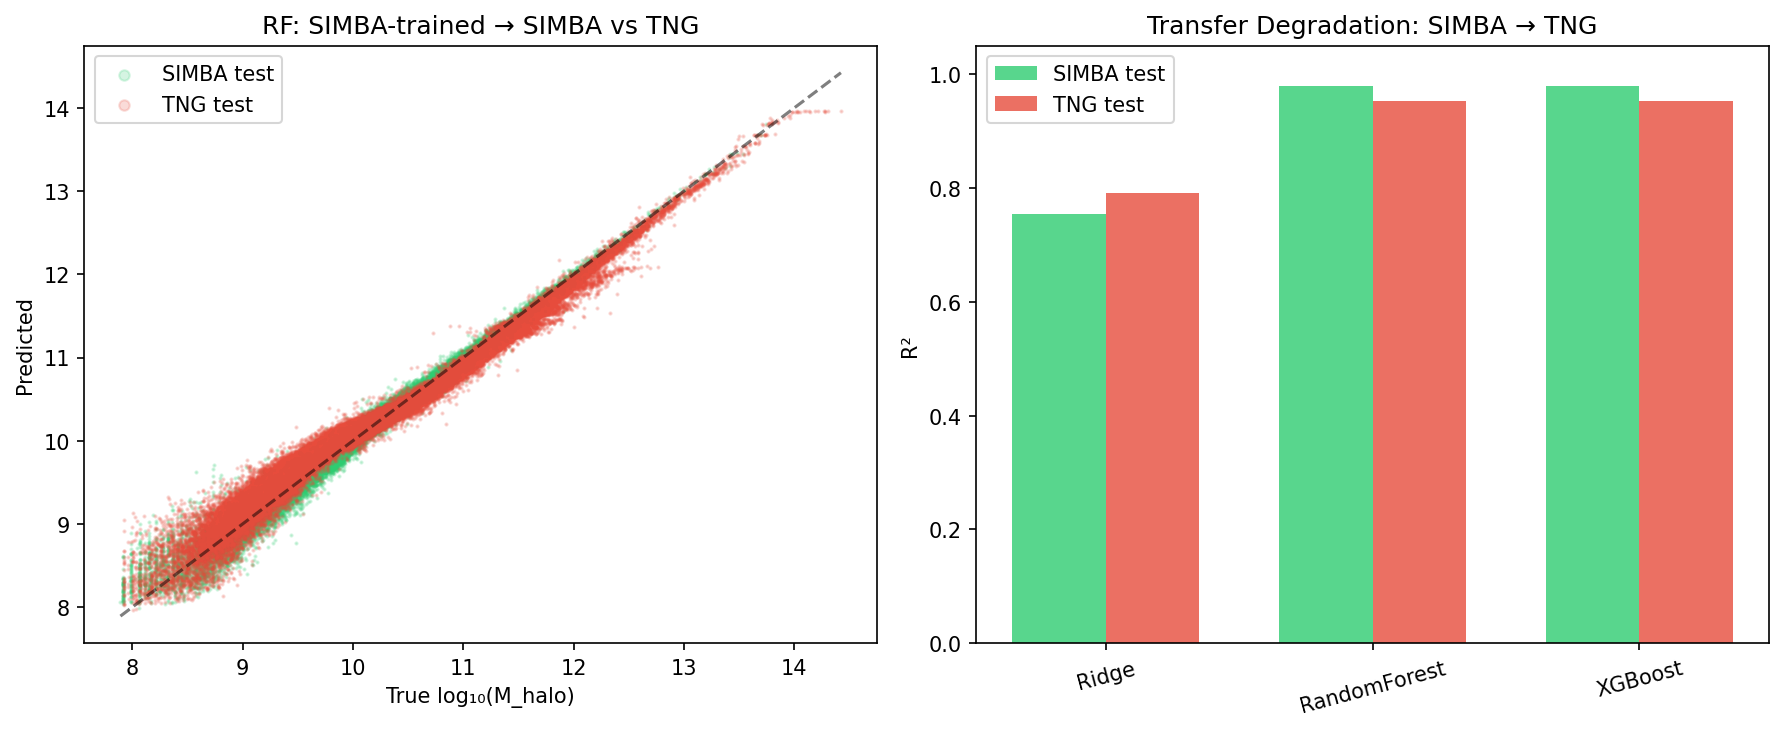
\includegraphics[width=0.90\textwidth]{step9_transfer/transfer_comparison.png}
  \caption{Cross-simulation transfer evaluation.  Left: predicted vs.\ true $\logMhalo$ for SIMBA-trained models evaluated on TNG.  Right: $R^2$ comparison between in-distribution (SIMBA) and out-of-distribution (TNG) evaluation.}
  \label{fig:transfer}
\end{figure}


% ~~~~~~~~~~~~~~~~~~~~~~~~~~~~~~~~~~~~~~~~~~~~~~~~~~~~~~~~~~~~~~~~~~~~~~~~~~~~
%  SECTION 9: DISCUSSION & CONCLUSION
% ~~~~~~~~~~~~~~~~~~~~~~~~~~~~~~~~~~~~~~~~~~~~~~~~~~~~~~~~~~~~~~~~~~~~~~~~~~~~
\section{Discussion and Conclusion}
\label{sec:discussion}

This work has presented an end-to-end pipeline for predicting dark matter halo mass from baryonic galaxy properties using the CAMELS simulation suite.  We summarise the key findings and their implications:

\begin{enumerate}[nosep]
  \item \textbf{Velocity dispersion is the overwhelmingly dominant predictor.}  Across all model classes and interpretability methods---linear coefficients ($\beta = +0.494$), RF impurity importance (80.5\%), SHAP ($\overline{|\phi|} = 0.531$~dex), and PySR (first term discovered)---$\sigmav$ consistently emerges as the single most informative feature.  This is a direct empirical recovery of the virial theorem from tabular data.
  
  \item \textbf{The stellar-to-halo mass relation is recovered.}  Stellar mass is the second-ranked feature in all analyses, consistent with the well-established SHMR in the astrophysical literature.
  
  \item \textbf{Non-linearity is critical.}  Tree models ($R^2 = 0.980$) and the MLP ($R^2 = 0.978$) vastly outperform the linear baseline ($R^2 = 0.754$), confirming strong non-linear structure in the baryonic$\rightarrow$halo mass mapping that cannot be captured by additive linear combinations.
  
  \item \textbf{A compact analytic formula captures 95\% of the variance.}  PySR discovered $\hat{y} = 0.833\,\ln(\sigmav - 3.644) + \sqrt{\sqrt{r_{1/2}} + 53.85}$, achieving $R^2 = 0.951$ with only two features and five constants---demonstrating that the essential physics can be expressed in closed form.
  
  \item \textbf{Models generalise across simulation suites.}  SIMBA-trained RF models evaluated on IllustrisTNG data degrade by only 2.7\% in $R^2$ (0.980~$\rightarrow$~0.952), confirming that the learned mapping is not an artefact of any single galaxy formation code.
  
  \item \textbf{Sample efficiency is high.}  RF achieves $R^2 = 0.978$ with only 5\% of the training data ($n \approx 8{,}000$), indicating that the primary signal is strong and easily learnable.
  
  \item \textbf{Spatial position carries no predictive power.}  As expected from cosmological homogeneity within the simulation box, position coordinates have $|r| < 0.013$ with the target, serving as a useful sanity check on the pipeline.
  
  \item \textbf{Mass-binned errors are largest at the extremes.}  Low-mass halos ($\logMhalo < 9$) and cluster-scale objects ($\logMhalo > 12$) exhibit 2--8$\times$ higher RMSE than the bulk population, reflecting intrinsic physical scatter in these regimes.
\end{enumerate}

\paragraph{Limitations.}
Several limitations should be acknowledged.  First, we use a single snapshot ($z = 0$), and the predictive accuracy and feature importance hierarchy may evolve with redshift as the relative contribution of different baryonic processes changes.  Second, the analysis is restricted to central subhalos; incorporating satellite galaxies would require modelling the additional complexity of orbital dynamics within a host halo.  Third, the features used here are derived from simulation catalogs with perfect knowledge; in an observational context, measurement noise, selection effects, and photometric/spectroscopic biases would degrade performance.

\paragraph{Future work.}
Natural extensions include: (i)~multi-redshift analysis to track the evolution of the $\sigmav$--$M$ relation and feature importance across cosmic time; (ii)~incorporation of observational mock catalogs with realistic noise models to assess the feasibility of applying these models to survey data; (iii)~graph neural network architectures that can leverage the spatial structure and connectivity of halos within the cosmic web; and (iv)~extension of the symbolic regression approach to discover redshift-dependent formulas of the form $\logMhalo = f(\sigmav, \Mstar, r_{1/2}; z)$.

\bigskip
\noindent
In summary, this pipeline demonstrates that dark matter halo mass can be predicted with $R^2 \geq 0.95$ from just two baryonic observables ($\sigmav$ and $r_{1/2}$), that the prediction generalises across simulation physics, and that the underlying relationship can be captured in a compact analytic formula rooted in fundamental astrophysical scaling relations.


% ~~~~~~~~~~~~~~~~~~~~~~~~~~~~~~~~~~~~~~~~~~~~~~~~~~~~~~~~~~~~~~~~~~~~~~~~~~~~
%  APPENDIX
% ~~~~~~~~~~~~~~~~~~~~~~~~~~~~~~~~~~~~~~~~~~~~~~~~~~~~~~~~~~~~~~~~~~~~~~~~~~~~
\appendix

\section{Full PySR Pareto Front}
\label{app:pareto}

Table~\ref{tab:full_pareto} lists all 12 equations on the Pareto front discovered by PySR.  Features: $x_0 = \sigmav$, $x_1 = \log_{10}(\Mstar + 1)$, $x_2 = r_{1/2}$.

\begin{table}[H]
  \centering
  \caption{Complete PySR Pareto front.  Score quantifies the improvement in log-loss per unit complexity increase from the previous equation.}
  \label{tab:full_pareto}
  \footnotesize
  \begin{tabular}{@{}rrrl@{}}
    \toprule
    \# & Complexity & Loss & Equation \\
    \midrule
    0  & 1  & 0.5429 & $9.986$ \\
    1  & 4  & 0.0447 & $\ln(x_0) + 6.948$ \\
    2  & 6  & 0.0425 & $\ln(x_0 - 1.281) + 7.027$ \\
    3  & 8  & 0.0368 & $0.816\,\ln(x_0 - 3.843) + 7.732$ \\
    4  & 11 & 0.0338 & $\ln(x_0 - 1.657) + 7.380 - 1.508 / \sqrt{x_2}$ \\
    5  & 12 & 0.0293 & $0.833\,\ln(x_0 - 3.644) + \sqrt{\sqrt{x_2} + 53.85}$ \\
    6  & 13 & 0.0290 & $0.796\,\ln(x_0 - 4.096) + \sqrt{\ln(x_2^2) + 54.67}$ \\
    7  & 14 & 0.0289 & $0.808\,\ln(x_0 - 3.871) + \sqrt{\sqrt{x_2} + 1.117 + 54.17}$ \\
    8  & 15 & 0.0281 & $\sqrt{\ln((1.535 - x_2)^2) + 54.50} + 0.803\,\ln(x_0 - 4.068)$ \\
    9  & 16 & 0.0281 & $\sqrt{\ln((x_2 - \ln x_0)^2) + 54.68} + 0.802\,\ln(x_0 - 4.163)$ \\
    10 & 17 & 0.0264 & $0.804\,\ln(x_0 - 4.191) + \sqrt{\ln\bigl((x_2 + 4.989 - x_1)^2\bigr) + 54.50}$ \\
    11 & 19 & 0.0264 & $\sqrt{\ln\bigl(((x_2 + 4.191 + 0.804) - x_1)^2\bigr) + 54.50} + 0.804\,\ln(x_0 - 4.191)$ \\
    \bottomrule
  \end{tabular}
\end{table}

\end{document}
